\documentclass[9pt,aspectratio=1610]{beamer}
\usepackage{booktabs}% better quality tables, https://ctan.org/pkg/booktabs
\usepackage{multirow}
\usepackage{array}%    additional options for table columns, https://ctan.org/pkg/array
\newcolumntype{C}[1]{>{\centering\let\newline\\\arraybackslash\hspace{0pt}}m{#1}}
\usepackage{tikz}
\tikzset{>=latex} % for LaTeX arrow head
\usetikzlibrary{matrix}
\usepackage{amsmath}
\usepackage{hhline}
\usepackage[table]{xcolor}
\usepackage[dvipsnames]{xcolor}
\usepackage{caption}
\usepackage{subcaption}
\usepackage{hyperref}
\usepackage{cite}
\usepackage{tcolorbox}
%\usepackage[style=ieee,maxbibnames=10,sorting=none,backend=biber]{biblatex}
%\addbibresource{./refs.bib}

\usepackage{palatino}
\usepackage{mathpazo}
\usepackage{helvet}
\usepackage{titlesec}


\usepackage{sty/hepparticles}
\usepackage{sty/heppennames2}

\newcommand{\Pgp}{\ensuremath{\pi}}
\newcommand{\PM}{\ensuremath{\mathrm{M}}}
\newcommand{\pt}{\ensuremath{p_T}}
\newcommand{\ptg}{\ensuremath{p_T^\PGg}}
\newcommand{\ptm}{\ensuremath{p_T^\PM}}
\newcommand{\jj}{\ensuremath{\mathrm{jj}}}
\newcommand{\jone}{\ensuremath{\mathrm{j1}}}
\newcommand{\jtwo}{\ensuremath{\mathrm{j2}}}
\newcommand{\Irelm}{\ensuremath{I_{\text{rel}}^{\Pgm}}}
\newcommand{\Itrk}{\ensuremath{I^{\text{trk}}(M)}}
\newcommand{\Ineu}{\ensuremath{I^{\text{neu}}(M)}}
\newcommand{\ItrkK}{\ensuremath{I^{\text{trk}}(\mathrm{trk}_1)}}
\newcommand{\mllhad}{\ensuremath{m_{\mathrm{M}\PGg}}}
\newcommand{\PGrz}{\ensuremath{\PGr^0}}
\newcommand{\PKstarz}{\ensuremath{\PKst^{0}}}
\newcommand{\Hgrho}{\PH\to\PGrz\PGg}
\newcommand{\Hgphi}{\PH\to\PGf\PGg}
\newcommand{\Hgkstar}{\PH\to\PKstarz\PGg}
\newcommand{\gphi}{\PGf\PGg}
\newcommand{\grho}{\PGrz\PGg}
\newcommand{\gkstar}{\PKstarz\PGg}
\newcommand{\ztoll}{\PZ\to\ell\ell}
\newcommand{\htomg}{\PH\to\PM\PGg}
\newcommand{\ggH}{\Pg\Pg\PH}
\newcommand{\WH}{\PW\PH}
\newcommand{\ZH}{\PZ\PH}
\newcommand{\zz}{\PZ\PZ^{*}}
\newcommand{\Hzz}{\PH\to\zz}
\newcommand{\ppc}{\Pp\Pp}
\newcommand{\mpipi}{\ensuremath{m_{\Pgp\Pgp}}}
\newcommand{\pippim}{\Pgpp\Pgpm}
\newcommand{\kpkm}{\PKp\PKm}
\newcommand{\mkk}{\ensuremath{m_{\PK\PK}}}
\newcommand{\mkpi}{\ensuremath{m_{\PK\Pgp}}}
\newcommand{\ea}{\epsilon\mathcal{A}}
\newcommand{\dbias}{\Delta_{\text{bias}}}
\newcommand{\mumupm}{\Pgmp\Pgmm}
\newcommand{\pgjpsi}{\PGg\PJGy}
\newcommand{\pgy}{\ensuremath{\PGg\PGy}(2S)\xspace}
\newcommand{\pgu}{\ensuremath{\PGg\PGU}(nS)\xspace}
\newcommand{\pgr}{\ensuremath{\PGg\PGrz}\xspace}
\newcommand{\pgf}{\ensuremath{\PGg\PGf}\xspace}
\newlength\cmsTabSkip\setlength{\cmsTabSkip}{1ex}
\providecommand{\cmsTable}[1]{\resizebox{\textwidth}{!}{#1}}
\captionsetup{labelformat=simple}
\hypersetup{
	colorlinks=true,
	linkcolor=blue,
	citecolor=blue,
	urlcolor=blue
}

\hypersetup{
	colorlinks=true,
	linkcolor=BlueViolet,
	filecolor=BlueViolet,      
	urlcolor=BlueViolet,
	pdftitle={HIG-23-005},
	pdfpagemode=FullScreen,
}

\newcommand{\krhl}[1]{\textbf{\LARGE\color{red}#1}}
\newcommand{\kbhl}[1]{\textbf{\LARGE\color{BlueViolet}#1}}
\newcommand{\kblhl}[1]{\textbf{\color{Black}#1}}
\newcommand{\khl}[1]{\textbf{\color{structure}#1}}
\newcommand{\ktodo}[1]{\colorbox{yellow!30}{{\color{red}\textsuperscript{\tiny FIX! }}#1}}
\newcommand{\kmfig}[2]{\includegraphics[#2]{figures/23-005-v07-marked-figs/#1.pdf}}
\newcommand{\ktmfig}[2]{\includegraphics[#2]{figures/23-004-v08-marked-figs/#1.pdf}}
\newcommand{\kmtab}[2]{\includegraphics[#2]{tables/23-005-v07-marked-tables/#1.pdf}}
\newcommand{\kblock}[2]{
	\begin{tcolorbox}[colback=Thistle!5,colframe=BlueViolet,arc=0.5pt,outer arc=0.5pt,left=2pt,right=2pt,title=#1]
		#2
	\end{tcolorbox}
}
\newcommand{\kaltblock}[2]{
	\begin{tcolorbox}[colback=Thistle!5,colframe=Apricot!90!Melon,arc=0.5pt,outer arc=0.5pt,left=2pt,right=2pt,title=#1]
		#2
	\end{tcolorbox}
}
\newcommand{\krblock}[2]{
	\begin{tcolorbox}[colback=Thistle!5,colframe=Bittersweet,arc=0.5pt,outer arc=0.5pt,left=2pt,right=2pt,title=#1]
		#2
	\end{tcolorbox}
}
\newcommand{\kgblock}[2]{
	\begin{tcolorbox}[colback=Thistle!5,colframe=ForestGreen,arc=0.5pt,outer arc=0.5pt,left=2pt,right=2pt,title=#1]
		#2
	\end{tcolorbox}
}
\newcommand{\kbblock}[2]{
	\begin{tcolorbox}[colback=Thistle!5,colframe=RoyalBlue,arc=0.5pt,outer arc=0.5pt,left=2pt,right=2pt,title=#1]
		#2
	\end{tcolorbox}
}

%%%
\usetheme{CambridgeUS}
\usecolortheme{dolphin}
\usefonttheme{professionalfonts}
\usefonttheme[onlymath]{serif}
\setbeamerfont{title}{series=\bfseries}
%\setbeamercolor{title}{fg=white,bg=darkred}
\setbeamercolor{frametitle}{fg=black}
\setbeamerfont{caption}{size=\tiny}
\setbeamertemplate{enumerate items}[default]
\setbeamercolor{insertsectionhead}{fg=black}
\setbeamertemplate{itemize items}[circle]
\setbeamertemplate{bibliography item}{\insertbiblabel}

\setbeamertemplate{footline}
{
	\leavevmode%
	\hbox{%
		\begin{beamercolorbox}[wd=.22\paperwidth,ht=2.25ex,dp=1ex,center]{author in head/foot}%
			\usebeamerfont{author in head/foot}\insertshortauthor
		\end{beamercolorbox}%
		\begin{beamercolorbox}[wd=.48\paperwidth,ht=2.25ex,dp=1ex,center]{title in head/foot}%
			\usebeamerfont{title in head/foot}\insertshorttitle
		\end{beamercolorbox}%
		\begin{beamercolorbox}[wd=.3\paperwidth,ht=2.25ex,dp=1ex,center]{date in head/foot}%
			\usebeamerfont{date in head/foot}\hspace*{1em}\insertshortdate\hspace*{3em}
			\insertframenumber{} / \inserttotalframenumber\hspace*{1ex}
		\end{beamercolorbox}}%
	\vskip0pt%
}
\AtBeginSection[]{
	\begin{frame}
		\vfill
		\centering
		\begin{beamercolorbox}[sep=8pt,center,shadow=false,rounded=true]{title}
			\usebeamerfont{title}\thesection. \insertsectionhead\par%
		\end{beamercolorbox}
		\vfill
	\end{frame}
}
%%%

%%% booktabs
\renewcommand{\arraystretch}{1.5}
%%%

\title[Approval Talk HIG-23-005]{{\color{Periwinkle}Approval Talk [HIG-23-005]}\\{\huge``Search for rare decays of the Higgs boson into a photon\\and a \(\rho^0\), \(\phi\) or \(K^{*0}\) meson"}}
\author[K. Yoon]{R. Covarelli\textsuperscript{1,2} \and M. Pelliccioni\inst{1} \and G. Umoret\inst{1,2}\\
	\and M. D'Alfonso\inst{3} \and G. Gomez Ceballos\inst{3} \and C. Paus\inst{3} \and \underline{K. Yoon}\inst{3}}
\institute[MIT]{\textsuperscript{1}INFN Torino, Turin, Italy \and \inst{2} Università degli Studi di Torino, Turin, Italy \and \inst{3} Massachusetts Institute of Technology, Cambridge, U.S.}
\date{March 19, 2024}

\pdfinfo{
	/Author (K. Yoon)
	/Title (HIG-23-005)
	/Subject (Approval Talk)
	/Keywords (Higgs Rare Decays, Htorhophik0stargamma)
	/Publisher (CMS)
}

\begin{document}

% Title
\begin{frame}[plain]
    \maketitle
\end{frame}

%%%%%% Outline %%%%%%
\begin{frame}{Outline}
	\begin{columns}
		\centering
		\begin{column}{0.9\textwidth}
			\kblhl{About this analysis}\dotfill\ref{fr:about}\\
			\vspace{1em}
			\kblhl{Introduction}\dotfill\ref{sec:intro}\\
			\kblhl{Analysis Strategy}\dotfill\ref{sec:anstrat}\\
			\kblhl{Triggers}\dotfill\ref{sec:trig}\\
			\kblhl{Simulated Samples}\dotfill\ref{sec:simsam}\\
			\kblhl{Event Selection}\dotfill\ref{sec:evsel}\\
			\kblhl{Multivariate Analysis Selection}\dotfill\ref{sec:mva}\\
			\kblhl{Signal \& Background Modeling}\dotfill\ref{sec:model}\\
			\kblhl{Systematic Uncertainties}\dotfill\ref{sec:syst}\\
			\kblhl{Results}\dotfill\ref{sec:res}\\
			\vspace{1em}
			\kblhl{Backup Slides}\dotfill\ref{sec:backup}\\
			\kblhl{References}\dotfill\ref{fr:refs}
		\end{column}
	\end{columns}
\end{frame}

% About
\begin{frame}{About this analysis}
	\label{fr:about}
	\kbhl{HIG-23-005}\\
	\vspace{1em}
	\textbf{Collaboration}
	\begin{itemize}
		\item Collaboration of \textbf{MIT} and \textbf{Torino} groups, targeting different Higgs production categories.
	\end{itemize}

	\textbf{Conveners}
	\begin{itemize}
		\item \textbf{ARC}: Anadi Canepa (chair), Stefan Spanier, Jian Wang, Angelo Giacomo Zecchinelli
		\item \textbf{CCLE}: Christoph Maria Ernst Paus
	\end{itemize}

	\textbf{Documentation}
	\begin{itemize}
		\item Relevant links: \href{https://cms.cern.ch/iCMS/analysisadmin/cadilines?id=2681&ancode=HIG-23-005&tp=an&line=HIG-23-005}{CADI}, \href{https://twiki.cern.ch/twiki/bin/view/CMS/HMesonGamma_QA}{TWiki}, \href{https://indico.cern.ch/event/1298068/\#29-pre-approval-of-hig-23-005}{Pre-Approval Talk}, \href{https://indico.cern.ch/event/1319601/\#21-unblinding-of-hig-23-005-se}{Unblinding Talk}
		\item Latest ANs (two individual + one combined):\\ \href{http://cms.cern.ch/iCMS/jsp/openfile.jsp?tp=draft&files=AN2022_004_v9.pdf}{AN-22-004} (MIT, v9), \href{http://cms.cern.ch/iCMS/jsp/openfile.jsp?tp=draft&files=AN2022_067_v10.pdf}{AN-22-067} (Torino, v10), and \href{http://cms.cern.ch/iCMS/jsp/openfile.jsp?tp=draft&files=AN2023_004_v7.pdf}{AN-23-004} (combined, v7)
	\end{itemize}
\end{frame}

%%%%%% 1. Section: Introduction %%%%%%
\begin{frame}
	\label{sec:intro}
	\vfill
	\centering
	\begin{beamercolorbox}[sep=8pt,center,shadow=false,rounded=true]{title}
		\usebeamerfont{title}\Huge Introduction \par%
	\end{beamercolorbox}
	\vfill
\end{frame}

% Motivations (table)
\begin{frame}{Motivations}
	\textbf{Higgs coupling with light quarks \((\PQu, \PQd, \PQs)\)}
	\begin{itemize}
		\item Suppressed couplings and large QCD background hamper direct searches.
		\item Class of decays suggested \(\htomg\), where \(\PM\) is a light-quark meson.
		\item \textit{In this analysis}, \(\PM=\PGf, \PGrz, \PKstarz\) are considered.
%		\item SM prediction of branching ratios of \(H\rightarrow \phi\PGg\) or \(\rho\PGg\) within reasonable reach (??)
%		\item ATLAS upper limit at \(95\)\% CL is \(\mathcal{O}(10^{-4})\) to \(\mathcal{O}(10^{-3})\).
%		\item \(K^*_0\) channel added as an extension of ditrack + gamma final state analyses.
	\end{itemize}
	\footnotesize
	\begin{table}[!ht]
		\centering
		\begin{tabular}[t]{|l|c|c|l|l|}
			\hline
			\multicolumn{1}{|c|}{\cellcolor{lightgray}\small Channel} & \cellcolor{lightgray}\small Coupling & \cellcolor{lightgray}\small SM \(\mathcal{BR}(\htomg)\)\\
			\hline
			
			% phi
			\multirow{2}{*}{\(\Hgphi\)} & \multirow{2}{*}{\(s\)} & \multirow{2}{*}{\((1.68\pm0.08) \times 10^{-5}\)\cite{K_nig_2015}} \\ & &\\
			\hline
			
			% rho
			\multirow{2}{*}{\(\Hgrho\)} & \multirow{2}{*}{\(u, d\)} & \multirow{2}{*}{\((2.31\pm0.11) \times 10^{-6}\)\cite{K_nig_2015}} \\ & & \\
			\hline
			
			% K0star
			\multirow{2}{*}{\(\Hgkstar\)} & & \tiny (Only available for \(\PH\to \PQd\PAQs + \PAQd\PQs\)) \\
			& \multirow{-2}{*}{\(d\&s\) (flavor-changing)} & \(1.19\times10^{-11}\) \cite{Aranda_2020} \\
			\hline
		\end{tabular}
		\caption{\(\htomg\) channels considered in this analysis with their respective couplings and predicted branching ratios.}
		\label{tab:Higgs_rare_decays}
	\end{table}
\end{frame}

% Motivations (flavor-conserving, flavor-changing)
\begin{frame}{Motivations}
	\begin{columns}
		\small
		\begin{column}{0.4\textwidth}
			{\large\khl{\(\htomg\)}}\\
			\vspace{1em}
			\textbf{1. Flavor-conserving probes}
			\begin{itemize}
				\item \textbf{Direct contribution}. The Higgs couples via Yukawa coupling to the quarks, one of which radiates a photon.
				\item \textbf{Indirect contribution}. The off-shell \(\PGg^*\) or \(Z^*\) produced in \(H\rightarrow \PGg\PGg^*, \PGg Z^*\) \textit{fragments} into a meson.
			\end{itemize}
			Direct and indirect contributions interfere destructively. Due to light quark masses, direct contribution is smaller than indirect. \textit{Direct contribution is sensitive to deviation from SM.} Branching ratios are \textit{typically} \(\mathcal{O}(10^{-5}\textup{--}10^{-6})\).\\
			\vspace{0.3em}
			\begin{itemize}
				\item \(\PGf\): \(\PQs\) quark coupling \textit{(diagrams above)}
				\item \(\PGrz\): \(\PQu\) and \(\PQd\) quark coupling
			\end{itemize}
			\vspace{0.5em}
			\textbf{2. Flavor-changing probe}
			\begin{itemize}
				\item \(\PKstarz\): flavor-changing \(\PQs\) and \(\PQd\) quarks via weak interaction \textit{(diagrams below)}
			\end{itemize}
		\end{column}
		\begin{column}{0.5\textwidth}
			\begin{figure}
				\centering
				\kmfig{fig1}{height=0.75\textheight}
				\caption{Feynman diagrams showing the different Higgs boson decay mechanisms into a photon and a light meson (top: \(\PGf\) meson; bottom: \(\PKstarz\) meson).}
			\end{figure}
		\end{column}
	\end{columns}
\end{frame}

%%%%%% 2. Section: Analysis Strategy %%%%%%
\begin{frame}
	\label{sec:anstrat}
	\vfill
	\centering
	\begin{beamercolorbox}[sep=8pt,center,shadow=false,rounded=true]{title}
		\usebeamerfont{title}\Huge Analysis Strategy \par%
	\end{beamercolorbox}
	\vfill
\end{frame}

% Strategy (final states)
\begin{frame}{Analysis Strategy}
	\begin{itemize}
		\item \khl{Final states}
		\begin{enumerate}
			\item High energy \textbf{photon}.
			\item High energy \textbf{di-track} from meson.
			\vspace{1em}
			\begin{figure}
				\centering
				\begin{subfigure}[b]{0.26\textwidth}
					\centering
					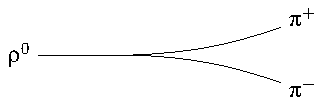
\includegraphics[width=\textwidth]{feynman-diagrams/rho_ditrack.pdf}
					\caption*{\footnotesize \(\mathcal{BR}(\PGrz\to\PGp^+\PGp^-) \sim100\%\)}
				\end{subfigure}
				\hfill
				\begin{subfigure}[b]{0.26\textwidth}
					\centering
					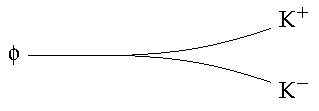
\includegraphics[width=\textwidth]{feynman-diagrams/phi_ditrack.pdf}
					\caption*{\footnotesize \(\mathcal{BR}(\PGf\to\PK^+\PK^-) \sim 49\%\)}
				\end{subfigure}
				\hfill
				\begin{subfigure}[b]{0.26\textwidth}
					\centering
					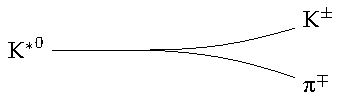
\includegraphics[width=\textwidth]{feynman-diagrams/kstar0_ditrack.pdf}
					\caption*{\footnotesize \(\mathcal{BR}(\PKstarz\to\PK^\pm\PGp^\mp) \sim 100\%\)}
				\end{subfigure}
				\hfill
				\caption{Di-track systems for the different mesons considered in this analysis.}
			\end{figure}
			\item Signal events extracted from \textbf{photon \& di-track invariant mass spectrum}.
		\end{enumerate}
	\end{itemize}
\end{frame}

% Strategy (production)
\begin{frame}{Analysis Strategy}
	\begin{itemize}
		\item \khl{Higgs Production Categories}
		\vspace{1em}
		\begin{columns}
			\centering
			\begin{column}{0.31\textwidth}
				\centering
				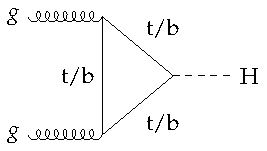
\includegraphics[height=0.25\textheight]{feynman-diagrams/ggH.pdf}\\
				\textbf{ggH}
				\begin{itemize}
					\item No \(\Pe/\PGm\).
%					\item Veto events with \(|\Delta\eta_{\jj}| > 3\)
				\end{itemize}
			\end{column}
			\begin{column}{0.31\textwidth}
				\centering
				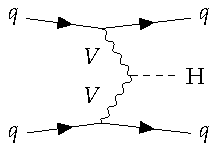
\includegraphics[height=0.25\textheight]{feynman-diagrams/VBF.pdf}\\
				\textbf{High-\(\ptg\) VBF}
				\begin{itemize}
					\item \(\ptg > 75\) GeV.
					\item No \(\Pe/\PGm\)
%					\item \(|\Delta\eta_{\jj}| > 3\), \(M_{JJ} > 400\) GeV
				\end{itemize}
				\vspace{1em}
				\textbf{Low-\(\ptg\) VBF}
				\begin{itemize}
					\item \(38 < \ptg < 75\) GeV.
					\item No \(\Pe/\PGm\)
%					\item \(|\Delta\eta_{\jj}| > 3\), \(M_{JJ} > 300\) GeV
				\end{itemize}
			\end{column}
			\begin{column}{0.31\textwidth}
				\centering
				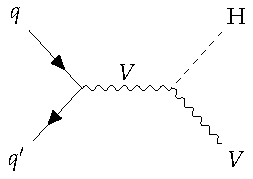
\includegraphics[height=0.25\textheight]{feynman-diagrams/VH.pdf}\\
				\textbf{VH (\(\mathbf{\PZ_{\Pl\Pl}\PH},\mathbf{\PW_{\Pl\PGn}\PH}\))}
				\begin{itemize}
					\item At least one \(\Pe/\PGm\).
					\item Also included is \(\mathbf{t\bar{t}H}\), accounting for \(\sim30\%\).
				\end{itemize}
			\end{column}
		\end{columns}
	\end{itemize}
\end{frame}

%%%%%% 3. Section: Triggers %%%%%%
\begin{frame}
	\label{sec:trig}
	\vfill
	\centering
	\begin{beamercolorbox}[sep=8pt,center,shadow=false,rounded=true]{title}
		\usebeamerfont{title}\Huge Triggers \par%
	\end{beamercolorbox}
	\vfill
\end{frame}

% Triggers
\begin{frame}{Triggers}
	\begin{itemize}
		\item \khl{High Level Triggers (HLT)}\\
		Three types of triggers are employed.
		\vspace{-1em}
	\end{itemize}
	\begin{columns}
		\begin{column}[t]{0.33\linewidth}
			\krblock{Tau-like trigger}{
				\textbf{Photon + jets with \(\PGt\)-ID}\\
				\hspace{2em}\textrightarrow\hspace{0.5em}\textbf{\color{Bittersweet}ggH, low-\(\ptg\) VBF}
				\begin{itemize}
					\item Photon \(\ptg>35\) GeV + tau-like jet \(\pt^\mathrm{j}>35\) GeV.
					\item Tau-leg similar to isolated di-track system.
					\item Luminosity:\\\(39.50\;\mathrm{fb^{-1}}\) (2018).
%					\item Trigger efficiencies derived from \(\PZ\to\PGmm\PGmp\).
				\end{itemize}
			}
			\vfill
		\end{column}%
		\hfill
		\begin{column}[t]{0.33\linewidth}
			\kgblock{VBF-dedicated trigger}{
				\textbf{High-\(\ptg\) photon + VBF-like jets}\\
				\hspace{2em}\textrightarrow\hspace{0.5em}\textbf{\color{ForestGreen}high-\(\ptg\) VBF}
				\begin{itemize}
					\item Photon \(\ptg>75\) GeV + di-jet with large \(M_{\jj}\) and \(\Delta\eta_\jj\).
					\item Active partly during 2016-17 and fully during 2018.
					\item Luminosities:\\\(28.2\;\mathrm{fb^{-1}}\) (2016), \(7.7 \;\mathrm{fb^{-1}}\) (2017), \(60\;\mathrm{fb^{-1}}\) (2018).
				\end{itemize}
			}
			\vfill
		\end{column}%
		\hfill
		\begin{column}[t]{0.33\linewidth}
			\kbblock{Leptonic trigger}{
				\textbf{Double or single lepton}\\
				\hspace{2em}\textrightarrow\hspace{0.5em}\textbf{\color{RoyalBlue}VH}
				\begin{itemize}
					\item Single or double-muon (electron) lowest \(\pt\) thresholds vary depending on year.
					\item To complement selection, triggers requiring a lepton and a photon is also used.
					\item Luminosity:\\\(138\;\mathrm{fb^{-1}}\) (2018).
				\end{itemize}
			}
			\vfill
		\end{column}
	\end{columns}
\end{frame}

% Triggers (efficiency)
\begin{frame}{Triggers}
	\begin{itemize}
		\item \khl{HLT Efficiencies and Scale Factors}\\
		Trigger efficiency \textbf{scale factor} defined as the ratio of data vs. MC efficiency.
		\begin{equation*}
			\text{SF} = \frac{\epsilon_\text{Data}}{\epsilon_\text{MC}}
		\end{equation*}\\
		\begin{itemize}
			\item For the tau-like trigger, Data = Single Muon, MC = Drell-Yan.\\ Photon-leg and tau-leg efficiencies measured separately.\\
%			{\small
%				\begin{align*}
%					\epsilon^{\mathrm{HLT}}_\PGg &= \frac{\text{HLT\_Mu17\_Photon30}\wedge\text{offline selection}\wedge\text{HLT\_IsoMu24}}{\text{offline selection}\wedge\text{HLT\_IsoMu24}}\\
%					\\
%					\epsilon^{\mathrm{HLT}}_\mathrm{TwoProngs} &= \frac{\text{HLT\_IsoMu24\_TwoProngs35}\wedge\text{offline selection}\wedge\text{HLT\_IsoMu24}}{\text{offline selection}\wedge\text{HLT\_IsoMu24}}
%			\end{align*}}
%			\vspace{0.5em}
			\item Modification on photon-leg added to reduce fake photon rate by forcing the photon to be a FSR.
		\end{itemize}		
	\end{itemize}
\end{frame}

% Triggers (figs-like)
\begin{frame}{Triggers}
	\begin{itemize}
		\item \khl{HLT Efficiencies and Scale Factors}\\
		Tau-like trigger efficiencies MC (blue) vs. Data (black).\\
		\vspace{0.5em}	
		\begin{figure}
			\centering
			\begin{subfigure}{0.45\linewidth}
				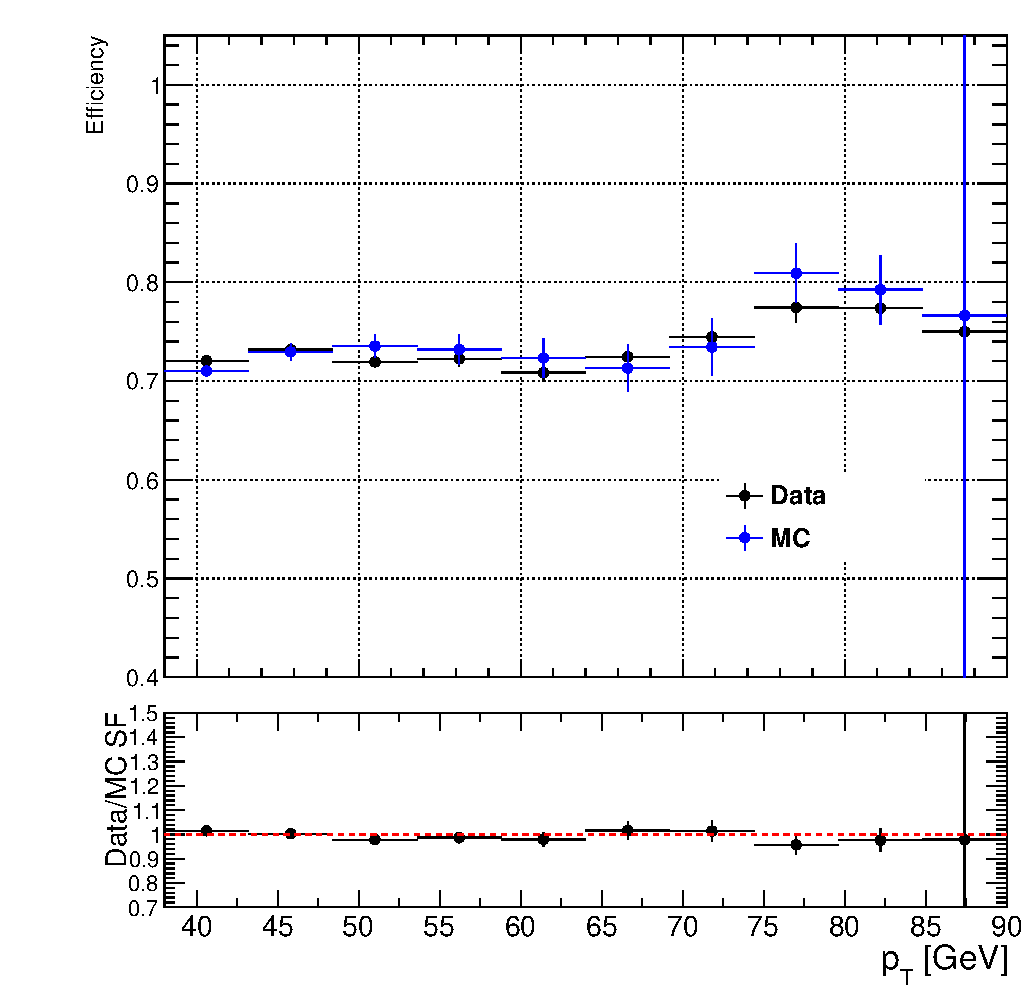
\includegraphics[width=\textwidth]{figures/misc/tau_trigger_photon_efficiencies.pdf}
				\vspace{-2em}
				\caption{Tau-like trigger photon-leg efficiencies for MC and data.}
			\end{subfigure}%
			\hfill
			\begin{subfigure}{0.45\linewidth}
				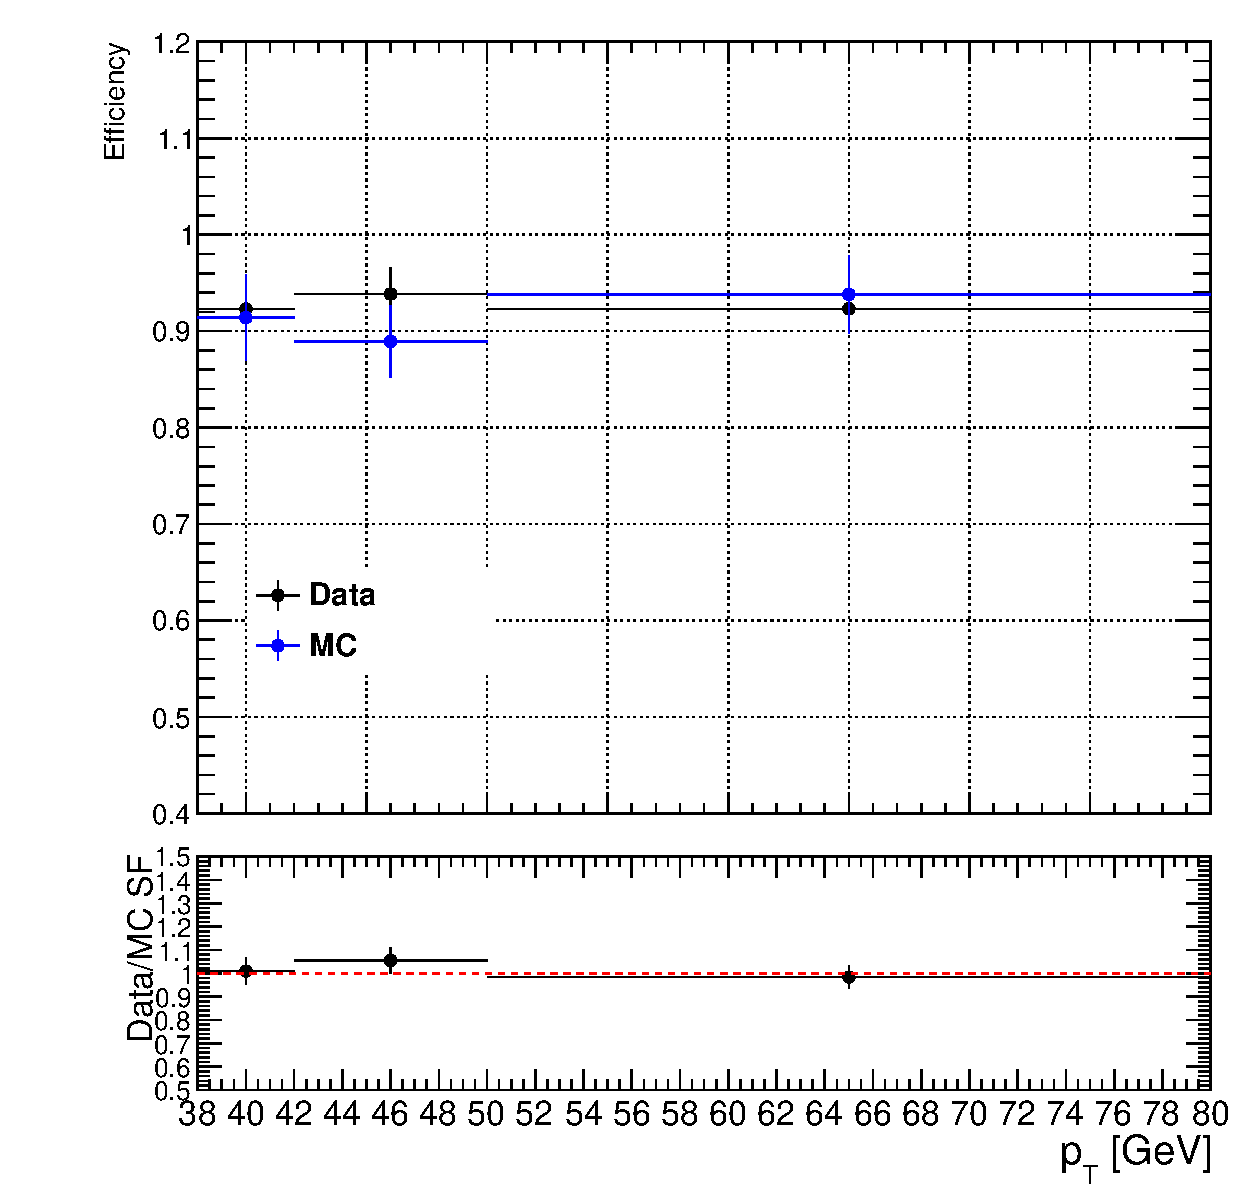
\includegraphics[width=\textwidth]{figures/misc/tau_trigger_two_prong_efficiencies.pdf}
				\vspace{-2em}
				\caption{Tau-like trigger tau-leg efficiencies for MC and data.}
			\end{subfigure}
			\vspace{-1em}
		\caption{Photon-leg and tau-leg efficiencies of the tau-like trigger.}
		\end{figure}
	\end{itemize}
\end{frame}

%%%%%% 4. Section: Simulated Samples %%%%%%
\begin{frame}
	\label{sec:simsam}
	\vfill
	\centering
	\begin{beamercolorbox}[sep=8pt,center,shadow=false,rounded=true]{title}
		\usebeamerfont{title}\Huge Simulated Samples \par%
	\end{beamercolorbox}
	\vfill
\end{frame}

% Simulated Samples (MC)
\begin{frame}{Simulated Samples}
	\begin{itemize}
		\item \khl{MC Generation}\\
		\vspace{0.5em}
		Gen-level: \texttt{POWHEG} (NLO) or \texttt{MADGRAPH5\_aMC@NLC} (LO)\\
		PDFs: \texttt{NNPDF3.1} (NNLO)\\
		Hadronization: \texttt{PYTHIA 8.212}
		\item SM processes considered in background simulation are\\
		\(\PGg\), \(\PW\to\Pl\PGn\), Drell-Yan \(\PZ\to\Pl\Pl\) with jets, \(\PQt\PAQt\), \(\PW\PGg\), and \(\PZ\PGg\).
		\item Cross sections for Higgs production:\\
		\hspace{2em}
		\begin{tabular}{l|l}
			Process & \(\sigma\) (fb)\\
			\hline
			ggH & 48580\\
			VBF & 3782\\
			W\(_{\Pl\PGn}\)H & 471\\
			Z\(_{\Pl\Pl}\)H & 77\\
			ggZ\(_{\Pl\Pl}\)H & 12
		\end{tabular}
	\end{itemize}
\end{frame}

% Simulated Samples (polarization)
\begin{frame}{Simulated Samples}
	\begin{columns}
		\begin{column}[b]{0.5\textwidth}
			\begin{itemize}
				\item \khl{Signal Simulation}\\
				\vspace{0.5em}
				\textbf{Polarization reweighting} of events.\\
				{\small
					Higgs is a scalar, and angular momentum conservation constrains the mesons to have transverse spin alignment in the \(\PH\to\PM\PGg\) process. \texttt{PYTHIA} simulates unpolarized decay products. Therefore, signal events are reweighted by \((3/2)\sin^2\theta\), where \(\theta\) is the angle between positive track in meson rest frame and meson flight direction in lab frame.
				}
			\end{itemize}
		\end{column}
		\begin{column}{0.5\textwidth}
			\begin{figure}
				\centering
				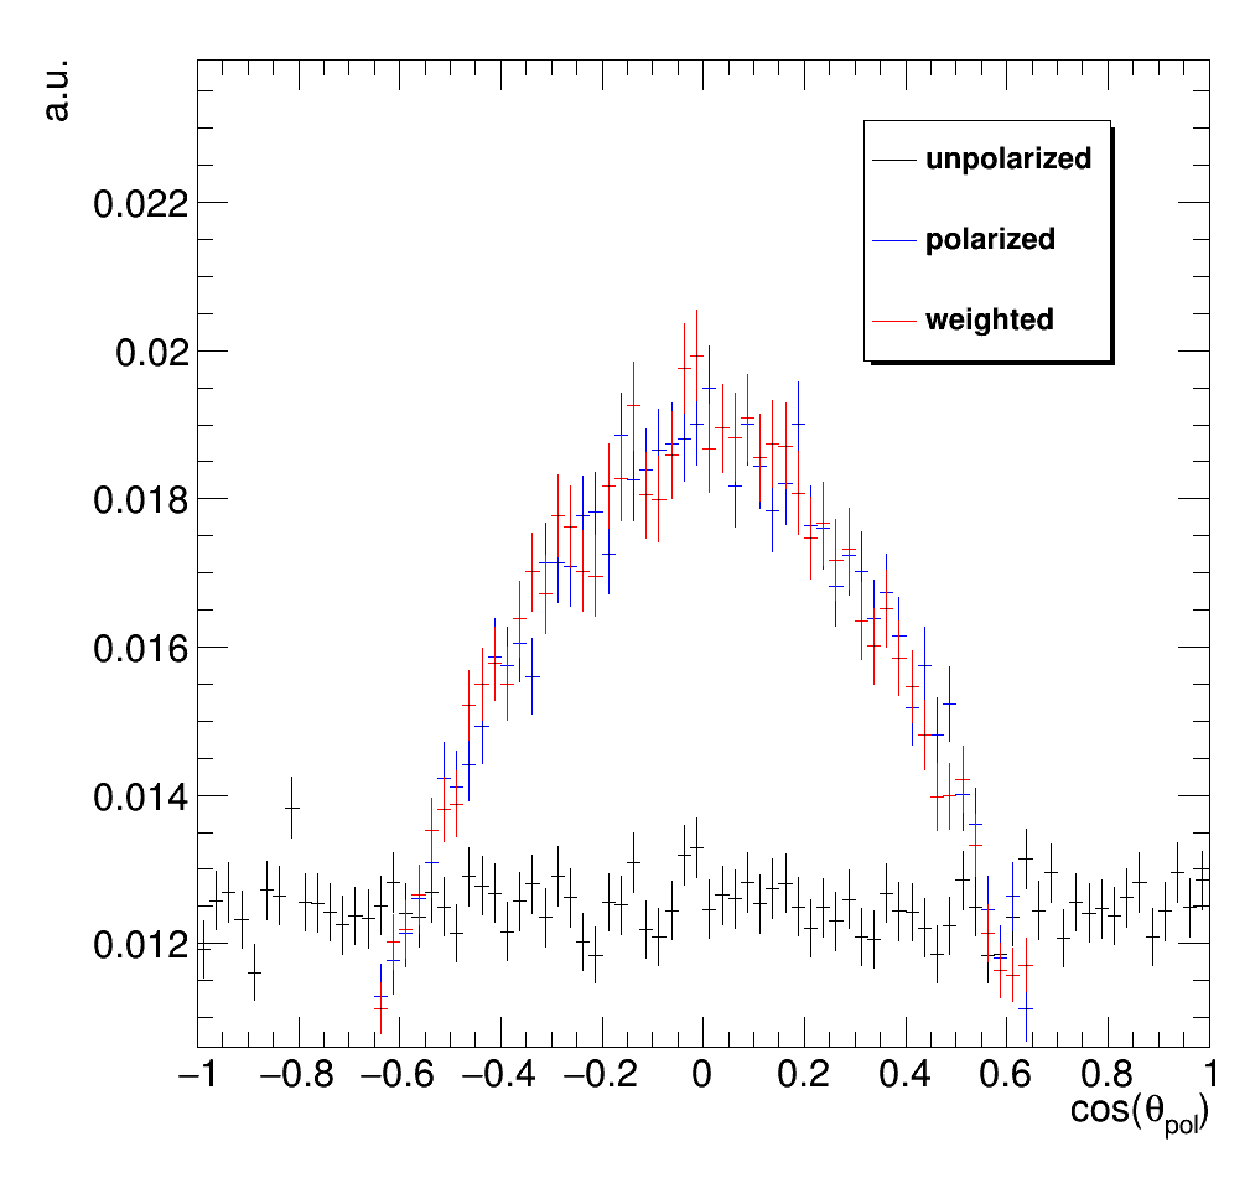
\includegraphics[width=0.85\textwidth]{figures/misc/polarization_angle_rho.pdf}
				\vspace{-1em}
				\caption{\(\cos\theta\) for the \(\rho\) meson decay. The black flat distribution illustrates the polarization angle within the centrally produced MC signal. The blue distribution portrays a privately generated MC signal wherein the accurate polarization was already incorporated. The red distribution results from reweighting the black distribution using the reweighting technique outlined in this section.}
			\end{figure}
		\end{column}
	\end{columns}
\end{frame}

%%%%%% 5. Section: Event Selection %%%%%%
\begin{frame}
	\label{sec:evsel}
	\vfill
	\centering
	\begin{beamercolorbox}[sep=8pt,center,shadow=false,rounded=true]{title}
		\usebeamerfont{title}\Huge Event Selection \par%
	\end{beamercolorbox}
	\vfill
\end{frame}

% Event Selection (photon selection)
\begin{frame}{Event Selection}
	\begin{itemize}
		\item \khl{Photon selection}
		\vspace{1em}
		\begin{table}[!ht]
			\centering
			\small
			\begin{tabular}{|l|c|c|c|c|}
				\hline
				& \multicolumn{1}{C{8em}}{\textbf{ggH}} & \multicolumn{1}{C{8em}}{\textbf{High-\(\mathbf{\ptg}\) VBF}} & \multicolumn{1}{C{8em}}{\textbf{Low-\(\mathbf{\ptg}\) VBF}} &  \multicolumn{1}{C{8em}|}{\textbf{VH}} \\
				\hline
				\(\ptg\) [GeV] & \multicolumn{1}{C{8em}}{\(> 38\)} & \multicolumn{1}{C{8em}}{\(> 75\)} & \multicolumn{1}{C{8em}}{\(38 < \ptg < 75\)} & \multicolumn{1}{C{8em}|}{\(> 40\)}\\
				\(|\eta^\PGg|\) & \multicolumn{1}{C{8em}}{\(< 2.1\)} & \multicolumn{1}{C{8em}}{\(< 1.4\)} & \multicolumn{1}{C{8em}}{\(< 2.1\)} & \multicolumn{1}{C{8em}|}{\(< 2.5\)}\\
				\(\PGg\)-ID signal eff. & \multicolumn{1}{C{8em}}{\(80\%\)} & \multicolumn{1}{C{8em}}{\(90\%\)} & \multicolumn{1}{C{8em}}{\(80\%\)} & \multicolumn{1}{C{8em}|}{\(90\%\)}\\
				\hline
			\end{tabular}
			\caption{Photon selection criteria across different production categories.}
		\end{table}
		\begin{itemize}
			\item \(\PGg\)-ID signal eff. = MVA-based selection ID \cite{photon_mvaid}
			\item \(\ptg\) and \(|\eta^\PGg|\) cuts based on trigger thresholds and barrel vs. endcap considerations.
			\item ggH/VBF: conversion veto, VH: pixel veto.
			\item Highest-\(\ptg\) photon chosen as candidate.
		\end{itemize}
	\end{itemize}
\end{frame}

% Event Selection (di-track)
\begin{frame}{Event Selection}
	\begin{itemize}
		\item \khl{Di-track system reconstruction}
		\begin{columns}
			\begin{column}{0.4\linewidth}
				\kblock{Track selection}{
					\begin{itemize}
						\item Originate from PV.
						\item Pass ``high purity" criteria.
					\end{itemize}}
				\kblock{Meson definition}{
					\begin{itemize}
						\item Pair of oppositely charged tracks.
						\item \(\pt > 5\) GeV, \(|\eta| < 2.5\).
						\item At least one track \(\pt > 20\) GeV.
				\end{itemize}}
			\end{column}
			\begin{column}{0.4\linewidth}
				\kblock{Invariant mass}{
					\begin{itemize}
						\item Di-track system invariant \textbf{mass windows and sidebands} (next slide).
						\item \(K^\pm\pi^\mp\) system: if both combinations exist, then the one closest to \(m_{\PKstarz}\) is selected.
						\item Reject events where \(\mkk\) consistent with \(m_{\PGp\PGp}/m_{\PK\PGp}\) and have higher \(\pt\), vice versa.
				\end{itemize}}
				\vfill
			\end{column}
		\end{columns}
	\end{itemize}
	\vspace{1em}
	\begin{center}
		\khl{Applies to all production categories.}
	\end{center}
\end{frame}

% Event Selection (di-track mass windows & sidebands)
\begin{frame}{Event Selection}
	\begin{itemize}
		\item \khl{Di-track system reconstruction}\\
		\vspace{1em}
		Mass windows applied to invariant mass of di-track system.
	\end{itemize}
	\vspace{1em}
	\begin{figure}[!h]
		\centering
		\begin{subfigure}[t]{0.31\linewidth}
			\kmfig{fig2-top-left}{width=\textwidth}
			{\footnotesize
				\begin{align*}
					\PGrz\text{ mass window: }& 0.62<\mpipi<0.92 \text{ GeV}\\
					\text{Sidebands: }& 0.50<\mpipi<0.62 \text{ GeV} \\
					& 0.92<\mpipi<1.00 \text{ GeV}
				\end{align*}
			}
		\end{subfigure}%
		\hfill
		\begin{subfigure}[t]{0.31\linewidth}
			\kmfig{fig2-top-right}{width=\textwidth}
			{\footnotesize
				\begin{align*}
					\PGf\text{ mass window: }& 1.008<\mkk<1.032 \text{ GeV}\\
					\text{Sidebands: }& 1.000<\mkk<1.008 \text{ GeV} \\
					& 1.032<\mkk<1.042\text{ GeV}
				\end{align*}
			}
		\end{subfigure}%
		\hfill
		\begin{subfigure}[t]{0.31\linewidth}
			\kmfig{fig2-bottom}{width=\textwidth}
			{\footnotesize
				\begin{align*}
					\PKstarz\text{ mass window: }& 0.84 < \mkpi < 0.94 \text{ GeV}\\
					\text{Sidebands: }& 0.80<\mkpi<0.84 \text{ GeV} \\
					& 0.94<\mkpi<1.00 \text{ GeV}
				\end{align*}
			}
		\end{subfigure}
		\caption{Di-track mass distribution in selected events in data, for the ggH category of the analysis, \(\grho\) (left), \(\gphi\) (middle) and \(\gkstar\) (right) channels. Vertical dashed lines represent the signal mass region borders.}
		{\footnotesize For more information on meson mass resolution, see backup slide \ref{fr:mesmassres}.}
	\end{figure} 
\end{frame}

% Event selection (di-track)
\begin{frame}{Event Selection}
	\begin{itemize}
		\item \khl{Di-track system selection}\\
		\vspace{1em}
		Define the relative \textbf{charged isolation} of the leading meson candidate,
		\begin{align*}
			I^{\mathrm{trk}}(M) = \frac{\ptm}{\ptm + {\color{Plum}\sum_{\mathrm{trk}}|\pt^{\mathrm{trk}}|}}\,,
		\end{align*}
		and the \textbf{neutral isolation} as
		\begin{align*}
			I^{\mathrm{neu}}(M) = \frac{\ptm}{\ptm + {\color{Plum}\sum_{\mathrm{neu}}|\pt^{\mathrm{neu}}|}}\,.
		\end{align*}
		\({\color{Plum}\sum_{trk/neu}|\pt^{trk/neu}|}\) {: \color{Plum}sum of charged/neutral track \(\pt\) within \(\Delta R = 0.3\)} of meson candidate.
		\vspace{1em}
		\begin{table}[!ht]
			\centering
			\small
			\begin{tabular}{|l|c|c|c|c|}
				\hline
				& \multicolumn{1}{C{8em}}{\textbf{ggH}} & \multicolumn{1}{C{8em}}{\textbf{High-\(\mathbf{\ptg}\) VBF}} & \multicolumn{1}{C{8em}}{\textbf{Low-\(\mathbf{\ptg}\) VBF}} &  \multicolumn{1}{C{8em}|}{\textbf{VH}} \\
				\hline
				\(p^M_T\) [GeV] & \multicolumn{1}{C{8em}}{\(> 38\)} & \multicolumn{1}{C{8em}}{\(> 30\)} & \multicolumn{1}{C{8em}}{\(> 38\)} & \multicolumn{1}{C{8em}|}{\(> 38\)}\\
				\(I^{trk}_M\) & \multicolumn{1}{C{8em}}{\(> 0.9\)} & \multicolumn{1}{C{8em}}{\(> 0.9\)} & \multicolumn{1}{C{8em}}{\(> 0.9\)} & \multicolumn{1}{C{8em}|}{\(> 0.8\)}\\
				\(I^{neu}_M\) & \multicolumn{1}{C{8em}}{\(> 0.8\)} & \multicolumn{1}{C{8em}}{-} & \multicolumn{1}{C{8em}}{-} & \multicolumn{1}{C{8em}|}{-}\\
				\hline
			\end{tabular}
			\caption{Di-track system criteria across different production categories.}
		\end{table}
%		\begin{itemize}
%			\item Highest-\(\pt\) meson chosen as candidate.
%		\end{itemize}
	\end{itemize}
\end{frame}

% Event Selection (event tagging)
\begin{frame}{Event Selection}
	\begin{itemize}
		\item \khl{Event tagging}
		\vspace{1em}
		\begin{table}[!ht]
			\centering
			\small
			\begin{tabular}{|l|c|c|c|c|}
				\hline
				& \multicolumn{1}{C{8em}}{\textbf{ggH}} & \multicolumn{1}{C{8em}}{\textbf{High-\(\mathbf{\ptg}\) VBF}} & \multicolumn{1}{C{8em}}{\textbf{Low-\(\mathbf{\ptg}\) VBF}} &  \multicolumn{1}{C{8em}|}{\textbf{VH}} \\
				\hline
				Event tagging & \multicolumn{1}{C{8em}}{Meson candidate within a jet with \(\pt^\mathrm{j} > 40\) GeV, tracks with \(\Delta R < 0.07\)} & \multicolumn{1}{C{8em}}{2 jets with \(\pt^{j} > 40\) GeV, \(m_{jj} > 400\) GeV, \(\eta_{jj} > 3\)} & \multicolumn{1}{C{8em}}{2 jets with \(\pt^{j} > 30, 20\) GeV, \(m_{jj} > 300\) GeV, \(\eta_{jj} > 3\)} & \multicolumn{1}{C{8em}|}{1 selected and isolated \(e/\mu\) or 2 selected \(e/\mu\) compatible with \(m_Z\)}\\
				\hline
			\end{tabular}
			\caption{Event tagging selection criteria across different production categories.}
		\end{table}
	\end{itemize}
\end{frame}

%%%%%% 6. Section: MVA Selection %%%%%%
\begin{frame}
	\label{sec:mva}
	\vfill
	\centering
	\begin{beamercolorbox}[sep=8pt,center,shadow=false,rounded=true]{title}
		\usebeamerfont{title}\Huge Multivariate Analysis Selection \par%
	\end{beamercolorbox}
	\vfill
\end{frame}

% MVA (overview)
\begin{frame}{Multivariate Analysis Selection}
	\begin{itemize}
		\item \khl{Multivariate Analysis (MVA) Overview}\\
		\kaltblock{Motivation}{
			Improvement of signal-to-background ratio in categories with backgrounds dominated by \(\PGg+\text{jet}\) and multijet events. \textrightarrow\hspace{0.35em}\textbf{ggH}, \textbf{low-\(\mathbf{\ptg}\) VBF}, and \textbf{high-\(\mathbf{\ptg}\) VBF} categories.
		}
		\kblock{Methodology}{
			\begin{itemize}
				\item BDT classifiers based on ROOT TMVA \cite{hoecker2009tmva}, optimized with the Gradient boosting method.
				\item Training and validation samples defined by \textbf{meson mass SR \& sidebands}.
				\item Signal \& Background events weighted by \(1/(\sigma M/M)\), where
				\begin{align*}
					\frac{\sigma M}{M} = \sqrt{\left(\frac{\sigma M}{M}\right)^2_{\mathrm{meson}} + \left(\frac{\sigma  E}{E}\right)^2_{\mathrm{\PGg}}}
				\end{align*}
				\item BDT classification is further split into \textbf{two sub-categories} (``cat0" and ``cat1") based on optimized discriminator threshold values to improve upper limit results.
			\end{itemize}
		}		
	\end{itemize}
\end{frame}

% MVA (variables)
\begin{frame}{Multivariate Analysis Selection}
	\begin{itemize}
		\item \khl{MVA Overview}\\
		\vspace{0.5em}
		Input variables:
		\begin{table}
			\centering
			\begin{tabular}{l | c | c | c }
				& \multicolumn{1}{C{8em}|}{\textbf{ggH}} & \multicolumn{1}{C{8em}|}{\textbf{High-\(\mathbf{\ptg}\) VBF}} & \multicolumn{1}{C{8em}}{\textbf{Low-\(\mathbf{\ptg}\) VBF}} \\
				\hline
				& & \(p^{M\PGg}_T\) & \(p^{M\PGg}_T\) \\
				Kinematics & \(p^{\PGg}_T\) & \(p^{\PGg}_T\) & \(p^{\PGg}_T\) \\
				& \(p^{M}_T\) & \(p^{M}_T/m_{M\PGg}\) & \(p^{M}_T/m_{M\PGg}\) \\
				& \(\eta_M\) & & \\
				\hline
				Charged Isolation & \(I^{\mathrm{trk}}(\mathrm{trk_1})\) & \(I^{\mathrm{trk}}(\PM)\) & \(I^{\mathrm{trk}}(\PM)\) \\
				\hline
				Photon ID & & \(\PGg\) mvaID & \(\PGg\) mvaID\\
				\hline
				& & \(M_{\jj}\) & \(M_{\jj}\) \\
				Jet-related & & \(\Delta\phi_{\jj}\) & \(\Delta\phi_{\jj}\) \\
				& & \(z^*\) & \(z^*\) \\
			\end{tabular}
			\caption{Input variables used for ggH and VBF categories.}
		\end{table}
		\vspace{-2em}
		{\hspace*{0pt}\hfill\footnotesize \(z^*\) is the Zeppenfeld variable, defined as \(z^*=|\eta_{\PM\PGg} - 0.5(\eta_\jone + \eta_\jtwo)/|\Delta\eta_\jj|\).}
	\end{itemize}
\end{frame}

% MVA (ggH)
\begin{frame}{Multivariate Analysis Selection}
	\begin{itemize}
		\item \khl{MVA: ggH category}
		\vspace{1em}
		\begin{itemize}
			\item Training samples\\
			\vspace{0.5em}
			\hspace{2em}\textbf{Signal}: MC-generated.\\
			\hspace{2em}\textbf{Background}: Data from meson mass sidebands.
			\vspace{1em}\\
			\item 4 input variables\\
			\vspace{0.5em}
			\begin{tabular}{|l | l|}
				\hline
				\(\ptg\) & photon \(\pt\)\\
				\(\ptm\) & meson \(\pt\)\\
				\(\eta_{\PM}\) & meson \(\eta\)\\
				\(I^{\mathrm{trk}}(\mathrm{trk_1})\) & leading-track charged isolation\\
				\hline
			\end{tabular}
			\vspace{1em}
			\item BDT sub-categories\\
			\hspace{2em}cat0: BDT-score \(>0.55\), optimized for max value of \(S/\sqrt{B}\).\\
			\hspace{2em}cat1: \(-0.4<\) BDT-score \(<0.55\)
		\end{itemize}
	\end{itemize}
\end{frame}

% MVA (ggH)
\begin{frame}{Multivariate Analysis Selection}
	\begin{itemize}
		\item \khl{MVA: ggH category}\\
		\vspace{1em}
		\begin{itemize}
			\item Training results:
		\end{itemize}
		\begin{figure}
			\centering
			\begin{subfigure}[t]{0.31\textwidth}
				\caption*{\footnotesize\(\Hgrho\)}
				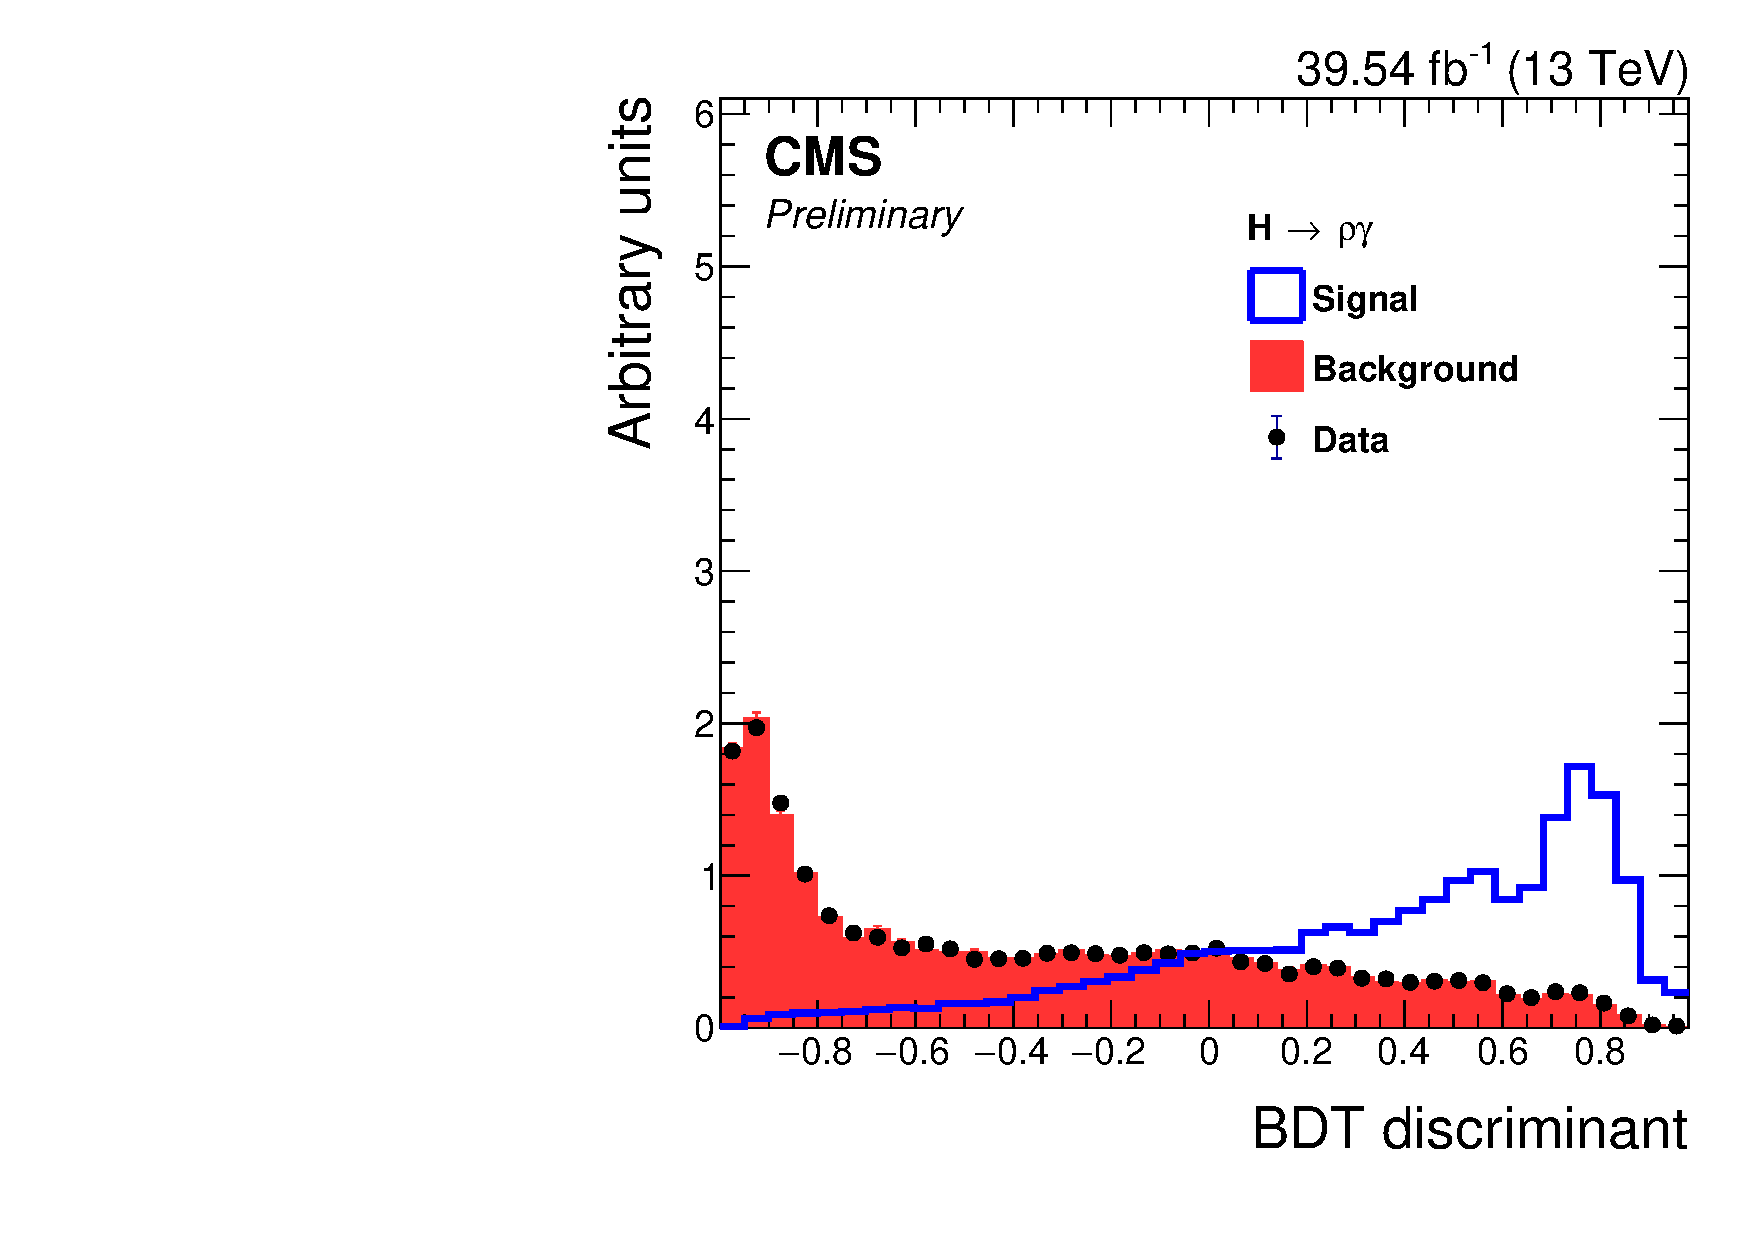
\includegraphics[width=\textwidth]{figures/misc/BDT_GF_Rho.pdf}
			\end{subfigure}%
			\hfill
			\begin{subfigure}[t]{0.31\textwidth}
				\caption*{\footnotesize\(\Hgphi\)}
				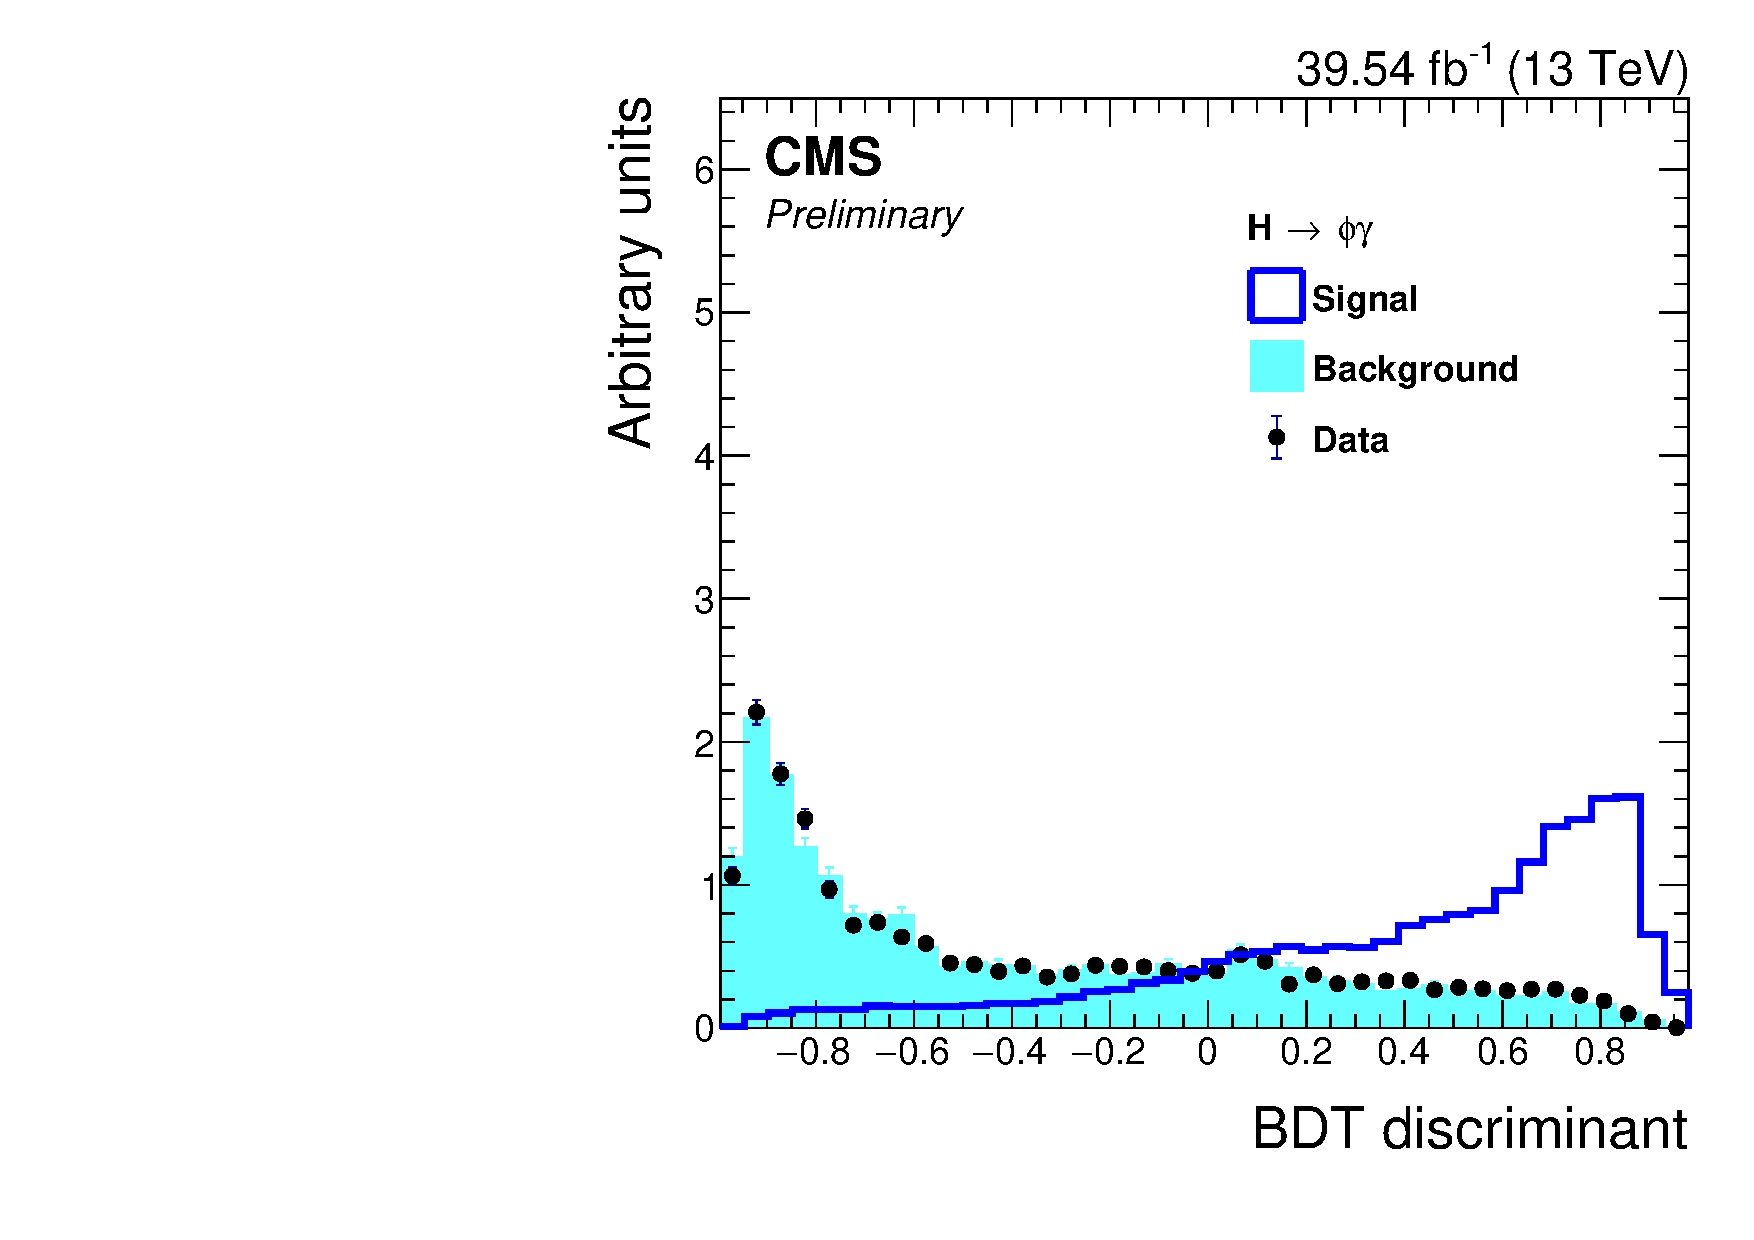
\includegraphics[width=\textwidth]{figures/misc/BDT_GF_Phi.pdf}
			\end{subfigure}%
			\begin{subfigure}[t]{0.31\textwidth}
				\caption*{\footnotesize\(\Hgkstar\)}
				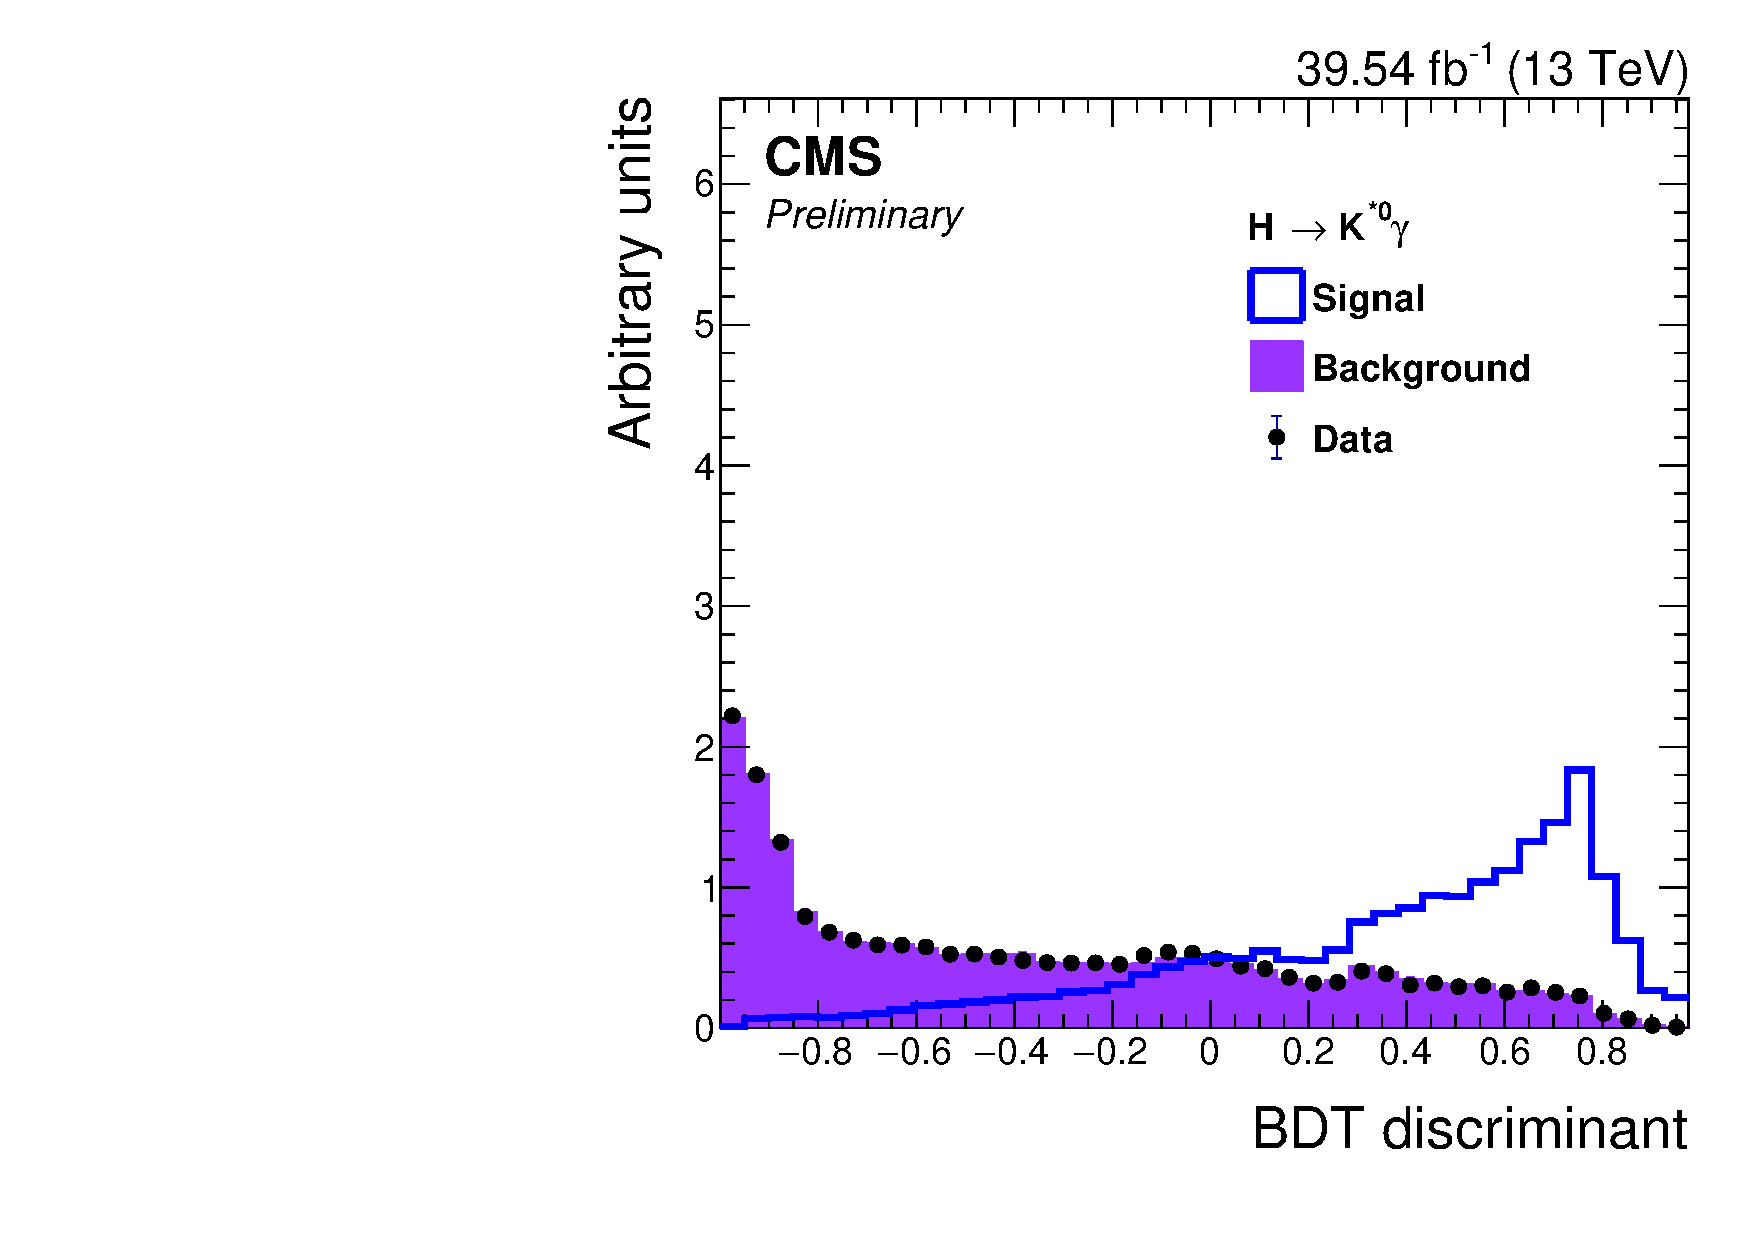
\includegraphics[width=\textwidth]{figures/misc/BDT_GF_K0s.pdf}
			\end{subfigure}
			\caption{BDT-score shown for the three decay channels of ggH.}
		\end{figure}
	\end{itemize}
\end{frame}

% MVA (VBF high&low)
\begin{frame}{Multivariate Analysis Selection}
	\begin{itemize}
		\item \khl{MVA: High \& Low-\(\ptg\) VBF categories}
		\vspace{1em}
		\begin{itemize}
			\item Training samples\\
			\vspace{0.5em}
			\hspace{2em}\textbf{Signal}: MC-generated.\\
			\hspace{2em}\textbf{Background}: \(\PGg\)+jets simulation and \(\PGg\) di-track events where the two tracks have the same charge.
			\vspace{1em}\\
			\item 8 input variables\\
			Variable that is correlated with Higgs candidate mass is divided by the mass.\\
			\vspace{0.5em}
			\hspace{2em}
			\begin{tabular}{|l | l|}
				\hline
				\(p^{\PM\PGg}_T\) & Higgs candidate \(\pt\)\\
				\(\ptg\) & photon \(\pt\)\\
				\(\ptm/m_{\PM\PGg}\) & meson \(\pt\) divided by Higgs candidate mass\\
				\(I^{\mathrm{trk}}(\PM)\) & meson charged isolation\\
				\(\PGg\) mvaID & photon identification discriminator\\
				\(M_{\jj}\) & di-jet invariant mass\\
				\(\Delta\phi_{\jj}\) & \(\Delta\phi\) of the two jets\\
				\(z*\) & Zeppenfeld variable\\
				\hline
			\end{tabular}
			\vspace{1em}
			\item BDT sub-categories\\
			\hspace{2em}cat0: BDT-score \(>0.7\), optimized for max value of \(S/\sqrt{B}\).\\
			\hspace{2em}cat1: \(-0.6<\) BDT-score \(<0.7\)
		\end{itemize}
	\end{itemize}
\end{frame}

% MVA (VBF high)
\begin{frame}{Multivariate Analysis Selection}
	\begin{itemize}
		\item \khl{MVA: High-\(\ptg\) category}\\
		\vspace{1em}
		\begin{itemize}
			\item Training results:
		\end{itemize}
		\begin{figure}
			\centering
			\begin{subfigure}[t]{0.31\textwidth}
				\caption*{\footnotesize\(\Hgrho\)}
				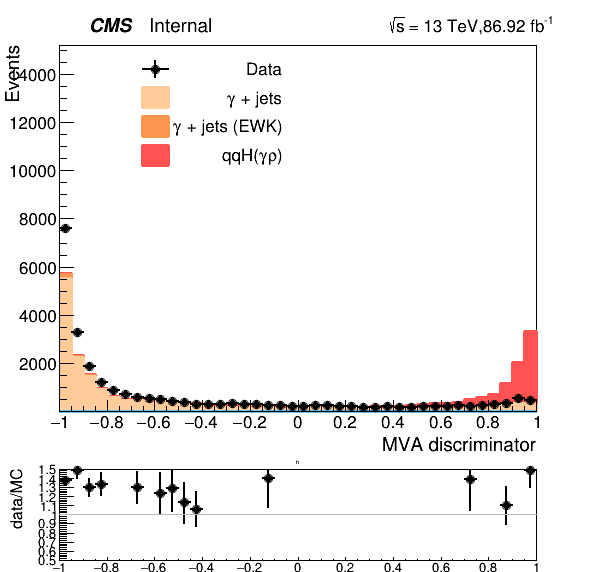
\includegraphics[width=\textwidth]{figures/misc/MVAdisc_VBFcat_RhoCat_all.png}
			\end{subfigure}%
			\hfill
			\begin{subfigure}[t]{0.31\textwidth}
				\caption*{\footnotesize\(\Hgphi\)}
				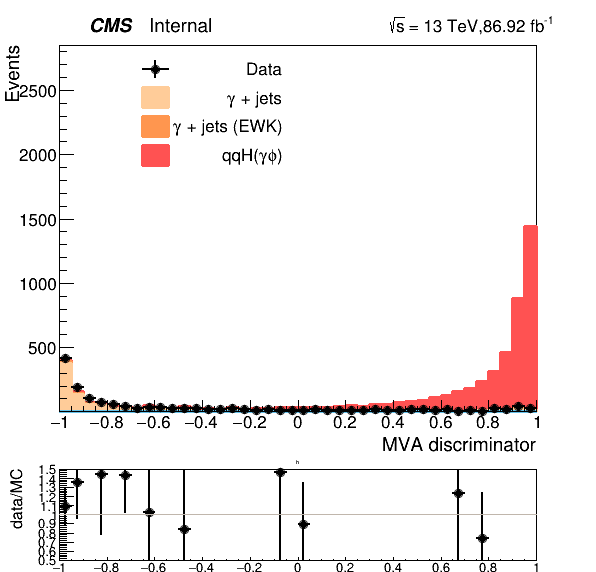
\includegraphics[width=\textwidth]{figures/misc/MVAdisc_VBFcat_PhiCat_all.png}
			\end{subfigure}%
			\begin{subfigure}[t]{0.31\textwidth}
				\caption*{\footnotesize\(\Hgkstar\)}
				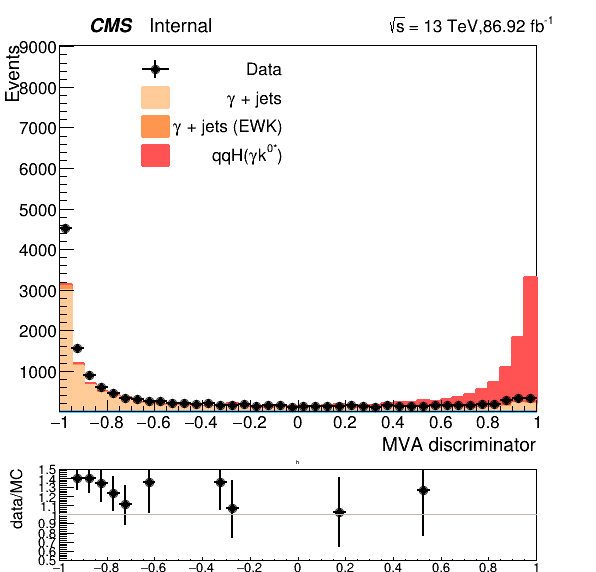
\includegraphics[width=\textwidth]{figures/misc/MVAdisc_VBFcat_K0StarCat_all.png}
			\end{subfigure}
			\caption{BDT-score shown for the three decay channels of high-\(\ptg\) VBF.}
		\end{figure}
	\end{itemize}
\end{frame}

% MVA (VBF low)
\begin{frame}{Multivariate Analysis Selection}
	\begin{itemize}
		\item \khl{MVA: Low-\(\ptg\) category}\\
		\vspace{1em}
		\begin{itemize}
			\item Training results:
		\end{itemize}
		\begin{figure}
			\centering
			\begin{subfigure}[t]{0.31\textwidth}
				\caption*{\footnotesize\(\Hgrho\)}
				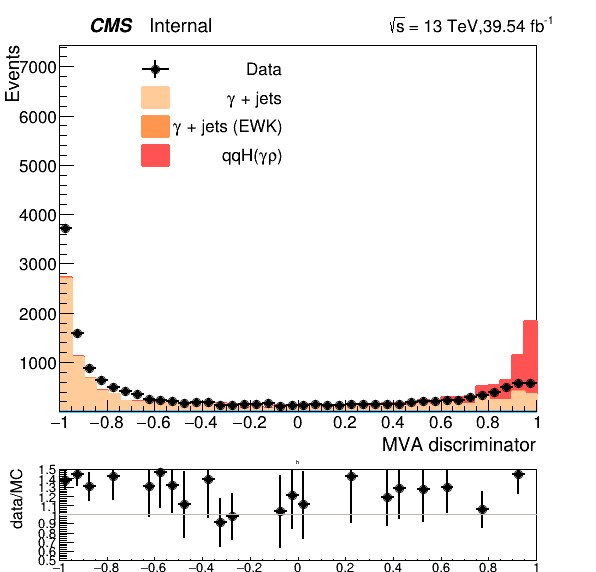
\includegraphics[width=\textwidth]{figures/misc/MVAdisc_VBFcatlow_RhoCat_12018.png}
			\end{subfigure}%
			\hfill
			\begin{subfigure}[t]{0.31\textwidth}
				\caption*{\footnotesize\(\Hgphi\)}
				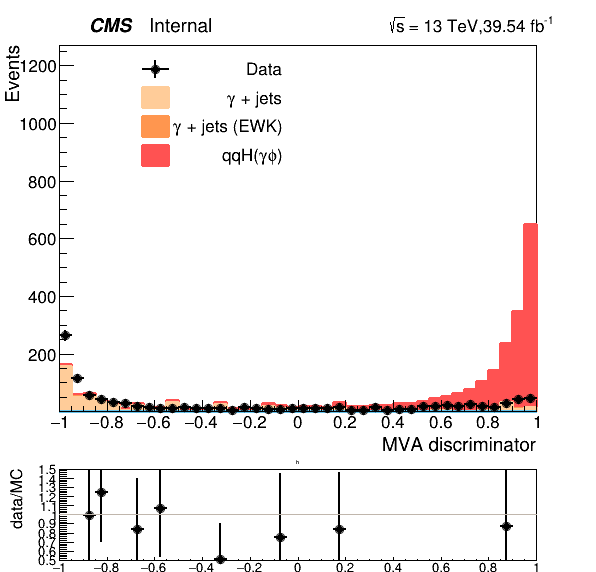
\includegraphics[width=\textwidth]{figures/misc/MVAdisc_VBFcatlow_PhiCat_12018.png}
			\end{subfigure}%
			\begin{subfigure}[t]{0.31\textwidth}
				\caption*{\footnotesize\(\Hgkstar\)}
				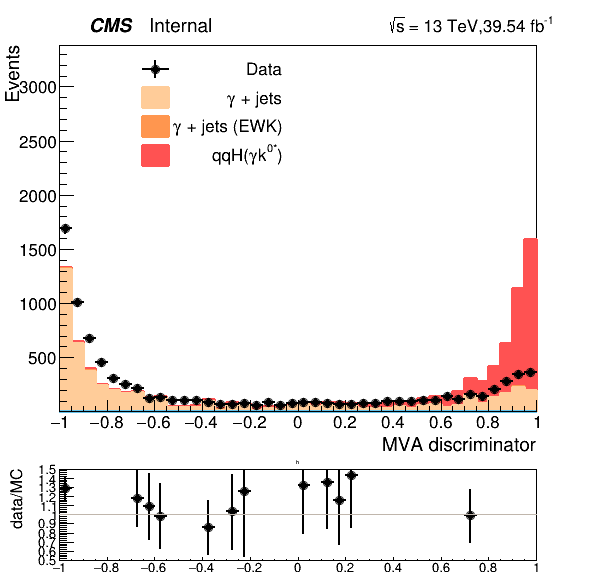
\includegraphics[width=\textwidth]{figures/misc/MVAdisc_VBFcatlow_K0StarCat_12018.png}
			\end{subfigure}
			\caption{BDT-score shown for the three decay channels of low-\(\ptg\) VBF.}
		\end{figure}
	\end{itemize}
\end{frame}

% Event Selection (total summary)
\begin{frame}{Event Selection}
	
	\khl{Summary of Event Selection}
	\vspace{0.2em}
	\begin{figure}
		\centering
		\kmtab{table1}{height=0.75\textheight}
		\caption{Summary of the event selections, including both common and category-specific selections.}
	\end{figure}
\end{frame}

%%%%%% 7. Section: Modeling %%%%%%
\begin{frame}
	\label{sec:model}
	\vfill
	\centering
	\begin{beamercolorbox}[sep=8pt,center,shadow=false,rounded=true]{title}
		\usebeamerfont{title}\Huge Signal \& Background Modeling \par%
	\end{beamercolorbox}
	\vfill
\end{frame}

% Signal modeling
\begin{frame}{Signal modeling}
	\begin{itemize}
		\item Signal events extracted from the distribution of the \khl{reconstructed Higgs boson mass}.
		\item Analytic function: \textbf{two-tailed Crystal Ball(TTCB)}.
		\begin{align*}
			\footnotesize
			\label{eq:ttcb}
			\mathrm{TTCB}(t) = \left\{
			\begin{array}{l l}
				e^{-t^2/2}, & \mathrm{for}~~-\alpha_L<t<\alpha_R\\
				(\frac{n_L}{|\alpha_L|})^{n_{L}}e^{-\alpha_L^2/2}(\frac{n_L}{|\alpha_L|}-|\alpha_L|-t)^{-n_{L}}, & \mathrm{for}~~t\leq-\alpha_L\\
				(\frac{n_R}{|\alpha_R|})^{n_{R}}e^{-\alpha_R^2/2}(\frac{n_R}{|\alpha_R|}-|\alpha_R|+t)^{-n_{R}}, & \mathrm{for}~~t\geq\alpha_L\\
			\end{array} \right.
		\end{align*}
		\item Fitted via unbinned likelihood to simulated signal events.
		\vspace{0.5em}
		\begin{figure}
			\centering
			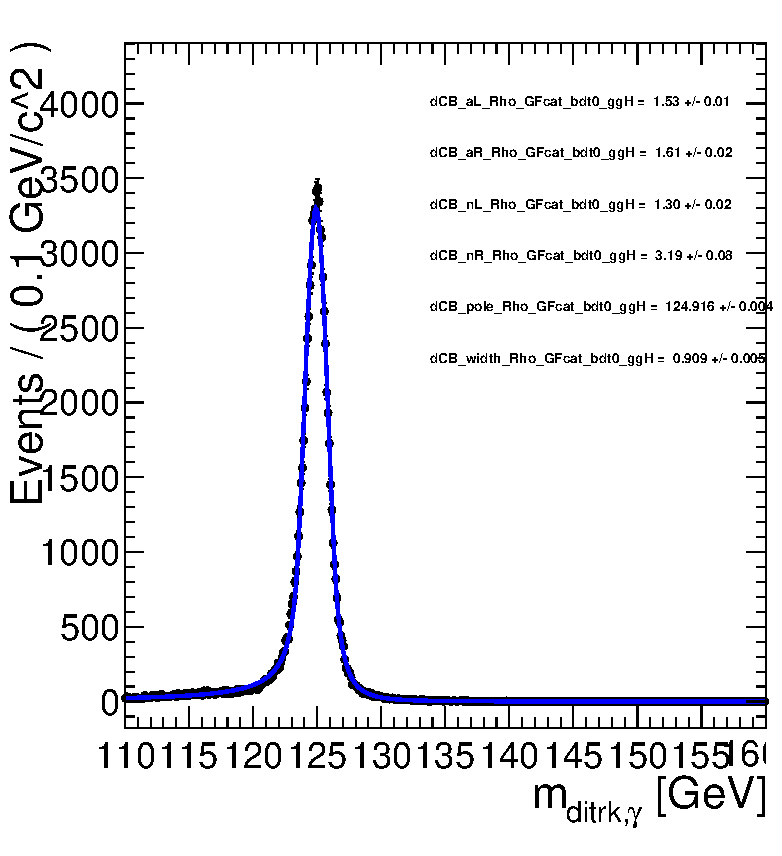
\includegraphics[height=0.52\textheight]{figures/misc/signal_ggH_Rho_cat0.pdf}
			\vspace{-1em}
			\caption{Example fitting of the TTCB function to the \(\Hgrho\) selected signal samples from BDT cat0 in the ggH category.}
		\end{figure}
	\end{itemize}
\end{frame}

% Background modeling
\begin{frame}{Background modeling}
	\begin{itemize}
		\item Analytic functions: \textbf{Chebychev} polynomials (main), \textbf{Bernstein} polynomials and \textbf{exponential} series (determination of shape uncertainties).
		\item Fitting region defined as \(m_{M\PGg}\) sidebands.\\
		\begin{itemize}
			\item ggH category: \(110 < m_{M\PGg} < 120\) GeV \& \(130 < m_{M\PGg} < 160\) GeV. 
			\item VBF categories (high \& low \(\ptg\)): \(100 < m_{M\PGg} < 120\) GeV \& \(130 < m_{M\PGg} < 170\) GeV.
			\item VH category: \(100 < m_{M\PGg} < 120\) GeV \& \(130 < m_{M\PGg} < 150\) GeV.
		\end{itemize}
		\item Degree of polynomial determined with \textbf{F-test}.
		\item \textbf{Bias studies} performed.
	\end{itemize}
\end{frame}

%%%%%% 8. Section: Systematic Uncertainties %%%%%%
\begin{frame}
	\label{sec:syst}
	\vfill
	\centering
	\begin{beamercolorbox}[sep=8pt,center,shadow=false,rounded=true]{title}
		\usebeamerfont{title}\Huge Systematic Uncertainties \par%
	\end{beamercolorbox}
	\vfill
\end{frame}

% Systematic uncertainties
\begin{frame}{Systematic Uncertainties}
	Signal uncertainty
	\begin{table}
		\small
		\begin{tabular}{l|l}
			\hline
			\textbf{Integrated Luminosity} & 2.5\% (2016), 2.3\% (2017), and 2.5\% (2018)\\
			\hline
			\textbf{Total inelastic cross section} & 4.6\%\\
			\hline
			\textbf{Trigger efficiencies} & VBF-dedicated trigger, 2.2-3.4\% (photon-leg)
			and 5.3-5.6\% (di-jet)\\
			\hline
			\textbf{Photon ID efficiencies} & Up to 1.5\%, \(\pt\) and \(\eta\) dependent\\
			\hline
			\textbf{Tracking efficiency} & 4.6\% (2.3\% per track)\\
			\hline
			\textbf{Muon/Electron ID} & Less than 1.0\% (muons) / 1.5\% (electrons)\\
			\hline
			\textbf{Meson Charged/Neutral Isolation Efficiencies} & 1.7-2.8 \%, depending on search channel and isolation type\\
			\hline
			\textbf{JEC \& JES} & Up to 3.5\% in VBF, negligible in ggH\\
			\hline
			\textbf{QCD renormalization and factorization} & 0.4\% (VBF), 0.7\% (WH), 3.8\% (ZH), and 2.6\% (\(\mathrm{t\bar{t}H}\))\\
			\hline
			\textbf{PDF \& \(\alpha_S\)} & 1.6-3.2\%, depending on Higgs production\\
			\hline
			\textbf{Parton shower modeling} & \(\mathcal{O}(0.1\%)\)\\
			\hline
		\end{tabular}
		\caption{Table of systematic uncertainties.}
	\end{table}

	Background shape uncertainty measured via \textbf{discrete profiling method}.
\end{frame}

%%%%%% 9. Section: Results %%%%%%
\begin{frame}
	\label{sec:res}
	\vfill
	\centering
	\begin{beamercolorbox}[sep=8pt,center,shadow=false,rounded=true]{title}
		\usebeamerfont{title}\Huge Results \par%
	\end{beamercolorbox}
	\vfill
\end{frame}

% Signal & Background fits (ggH cat0)
\begin{frame}{Signal \& Background Post-fit Distributions}
	\begin{itemize}
		\item \khl{ggH categories}
	\end{itemize}
	\begin{figure}
		\centering
		\begin{subfigure}[t]{0.31\textwidth}
			\kmfig{fig3-top-left}{width=\textwidth}
			\caption*{\footnotesize \(\Hgrho\), ggH cat0}
		\end{subfigure}%
		\hfill
		\begin{subfigure}[t]{0.31\textwidth}
			\kmfig{fig3-middle-left}{width=\textwidth}
			\caption*{\footnotesize \(\Hgphi\), ggH cat0}
		\end{subfigure}%
		\hfill
		\begin{subfigure}[t]{0.31\textwidth}
			\kmfig{fig3-bottom-left}{width=\textwidth}
			\caption*{\footnotesize \(\Hgkstar\), ggH cat0}
		\end{subfigure}
		\caption{Post-fit \(m_{\PM\PGg}\) distributions in data and the background model for the ggH cat0 channels.}
	\end{figure}
\end{frame}

% Signal & Background fits (ggH cat 1)
\begin{frame}{Signal \& Background Post-fit Distributions}
	\begin{itemize}
		\item \khl{ggH categories}
	\end{itemize}
	\begin{figure}
		\centering
		\begin{subfigure}[t]{0.31\textwidth}
			\ktmfig{mass-postfit-GFcat-bdt1-Rho}{width=\textwidth}
			\caption*{\footnotesize \(\Hgrho\), ggH cat1}
		\end{subfigure}%
		\hfill
		\begin{subfigure}[t]{0.31\textwidth}
			\ktmfig{mass-postfit-GFcat-bdt1-Phi}{width=\textwidth}
			\caption*{\footnotesize \(\Hgphi\), ggH cat1}
		\end{subfigure}%
		\hfill
		\begin{subfigure}[t]{0.31\textwidth}
			\ktmfig{mass-postfit-GFcat-bdt1-K0s}{width=\textwidth}
			\caption*{\footnotesize \(\Hgkstar\), ggH cat1}
		\end{subfigure}
		\caption{Post-fit \(m_{\PM\PGg}\) distributions in data and the background model for the ggH cat1 channels.}
	\end{figure}
\end{frame}

% Signal & Background fits (VBF cat0)
\begin{frame}{Signal \& Background Post-fit Distributions}
	\begin{itemize}
		\item \khl{High-\(\ptg\) VBF categories}
	\end{itemize}
	\begin{figure}
		\centering
		\begin{subfigure}{0.31\textwidth}
			\kmfig{fig3-top-right}{width=\textwidth}
			\caption*{\footnotesize \(\Hgrho\), high-\(\ptg\) VBF cat0}
		\end{subfigure}%
		\hfill
		\begin{subfigure}{0.31\textwidth}
			\ktmfig{mass-postfit-VBFcat-bdt0-Phi}{width=\textwidth}
			\caption*{\footnotesize \(\Hgphi\), high-\(\ptg\) VBF cat0}
		\end{subfigure}%
		\hfill
		\begin{subfigure}{0.31\textwidth}
			\ktmfig{mass-postfit-VBFcat-bdt0-K0s}{width=\textwidth}
			\caption*{\footnotesize \(\Hgkstar\), high-\(\ptg\) VBF cat0}
		\end{subfigure}
		\caption{Post-fit \(m_{\PM\PGg}\) distributions in data and the background model for the high-\(\ptg\) VBF cat0 channels.}
	\end{figure}
\end{frame}

% Signal & Background fits (VBF cat 1)
\begin{frame}{Signal \& Background Post-fit Distributions}
	\begin{itemize}
		\item \khl{High-\(\ptg\) VBF categories}
	\end{itemize}
	\begin{figure}
		\centering
		\begin{subfigure}[t]{0.31\textwidth}
			\ktmfig{mass-postfit-VBFcat-bdt1-Rho}{width=\textwidth}
			\caption*{\footnotesize \(\Hgrho\), high-\(\ptg\) VBF cat1}
		\end{subfigure}%
		\hfill
		\begin{subfigure}[t]{0.31\textwidth}
			\ktmfig{mass-postfit-VBFcat-bdt1-Phi}{width=\textwidth}
			\caption*{\footnotesize \(\Hgphi\), high-\(\ptg\) VBF cat1}
		\end{subfigure}%
		\hfill
		\begin{subfigure}[t]{0.31\textwidth}
			\ktmfig{mass-postfit-VBFcat-bdt1-K0s}{width=\textwidth}
			\caption*{\footnotesize \(\Hgkstar\), high-\(\ptg\) VBF cat1}
		\end{subfigure}
		\caption{Post-fit \(m_{\PM\PGg}\) distributions in data and the background model for the high-\(\ptg\) cat1 channels.}
	\end{figure}
\end{frame}

% Signal & Background fits (VBFlow cat0)
\begin{frame}{Signal \& Background Post-fit Distributions}
	\begin{itemize}
		\item \khl{Low-\(\ptg\) VBF categories}
	\end{itemize}
	\begin{figure}
		\centering
		\begin{subfigure}{0.31\textwidth}
			\kmfig{fig3-bottom-right}{width=\textwidth}
			\caption*{\footnotesize \(\Hgrho\), low-\(\ptg\) VBF cat0}
		\end{subfigure}%
		\hfill
		\begin{subfigure}{0.31\textwidth}
			\ktmfig{mass-postfit-VBFcatlow-bdt0-Phi}{width=\textwidth}
			\caption*{\footnotesize \(\Hgphi\), low-\(\ptg\) VBF cat0}
		\end{subfigure}%
		\hfill
		\begin{subfigure}{0.31\textwidth}
			\ktmfig{mass-postfit-VBFcatlow-bdt0-K0s}{width=\textwidth}
			\caption*{\footnotesize \(\Hgkstar\), low-\(\ptg\) VBF cat0}
		\end{subfigure}
		\caption{Post-fit \(m_{\PM\PGg}\) distributions in data and the background model for the low-\(\ptg\) VBF cat0 channels.}
	\end{figure}
\end{frame}

% Signal & Background fits (VBFlow cat 1)
\begin{frame}{Signal \& Background Post-fit Distributions}
	\begin{itemize}
		\item \khl{Low-\(\ptg\) VBF categories}
	\end{itemize}
	\begin{figure}
		\centering
		\begin{subfigure}[t]{0.31\textwidth}
			\ktmfig{mass-postfit-VBFcatlow-bdt1-Rho}{width=\textwidth}
			\caption*{\footnotesize \(\Hgrho\), low-\(\ptg\) VBF cat1}
		\end{subfigure}%
		\hfill
		\begin{subfigure}[t]{0.31\textwidth}
			\ktmfig{mass-postfit-VBFcatlow-bdt1-Phi}{width=\textwidth}
			\caption*{\footnotesize \(\Hgphi\), low-\(\ptg\) VBF cat1}
		\end{subfigure}%
		\hfill
		\begin{subfigure}[t]{0.31\textwidth}
			\ktmfig{mass-postfit-VBFcatlow-bdt1-K0s}{width=\textwidth}
			\caption*{\footnotesize \(\Hgkstar\), low-\(\ptg\) VBF cat1}
		\end{subfigure}
		\caption{Post-fit \(m_{\PM\PGg}\) distributions in data and the background model for the low-\(\ptg\) cat1 channels.}
	\end{figure}
\end{frame}

% Signal & Background fits (VH)
\begin{frame}{Signal \& Background Post-fit Distributions}
	\begin{itemize}
		\item \khl{VH categories}
	\end{itemize}
	\begin{figure}
		\centering
		\begin{subfigure}[t]{0.31\textwidth}
			\ktmfig{mass-postfit-Vcat-Rho}{width=\textwidth}
			\caption*{\footnotesize \(\Hgrho\), VH}
		\end{subfigure}%
		\hfill
		\begin{subfigure}[t]{0.31\textwidth}
			\ktmfig{mass-postfit-Vcat-Phi}{width=\textwidth}
			\caption*{\footnotesize \(\Hgphi\), VH}
		\end{subfigure}%
		\hfill
		\begin{subfigure}[t]{0.31\textwidth}
			\ktmfig{mass-postfit-Vcat-K0s}{width=\textwidth}
			\caption*{\footnotesize \(\Hgkstar\), VH}
		\end{subfigure}
		\caption{Post-fit \(m_{\PM\PGg}\) distributions in data and the background model for the VH channels.}
	\end{figure}
\end{frame}

% Unblinded limits (methodology)
\begin{frame}{Upper Limits}
	\begin{itemize}
		\item \khl{Upper limits} on $\mathcal{B}(H\rightarrow\rho^0\PGg)$, $\mathcal{B}(H\rightarrow\phi\PGg)$, and $\mathcal{B}(\Hgkstar)$ set at 95\% CL.
		\item CLs profile-likelihood ratio used as test-statistics, with the asymptotic approximation.
		\item Systematic uncertainties treated as nuisance parameters. 
	\end{itemize}
\end{frame}

% Unblinded limits (bands)
\begin{frame}{Upper Limits}
	\begin{figure}
		\begin{subfigure}{.36\textwidth}
			\centering
			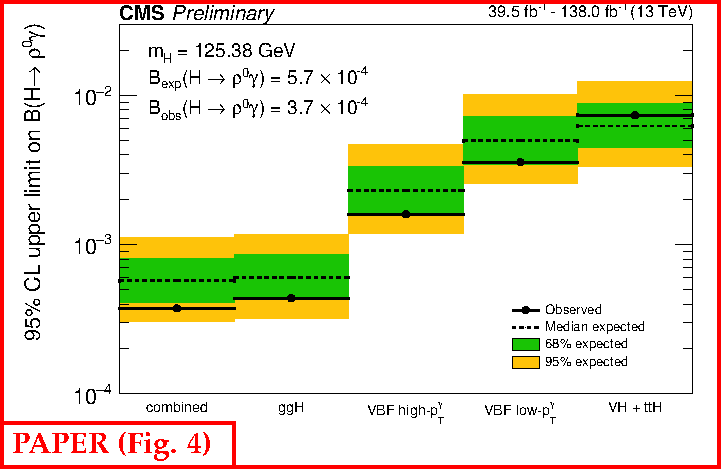
\includegraphics[width=\textwidth]{figures/23-005-v07-marked-figs/fig4-top-right.pdf}
		\end{subfigure}%
		\begin{subfigure}{.36\textwidth}
			\centering
			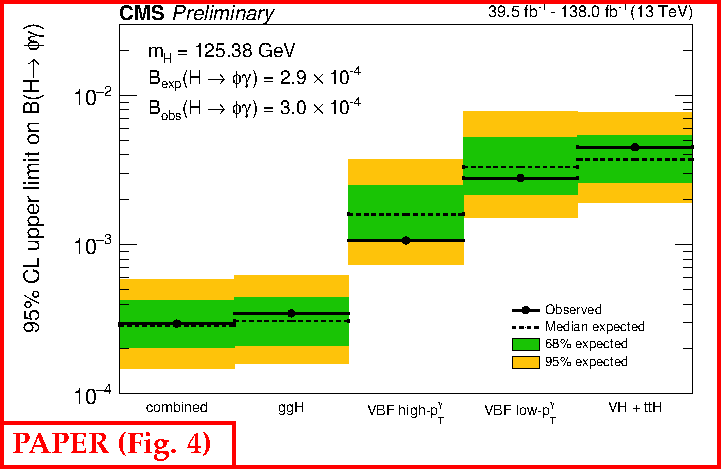
\includegraphics[width=\textwidth]{figures/23-005-v07-marked-figs/fig4-top-left.pdf}
		\end{subfigure}\\
		\begin{subfigure}{.36\textwidth}
			\centering
			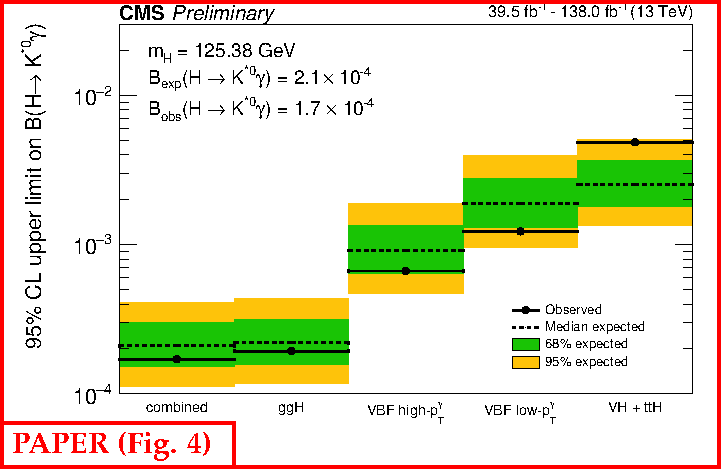
\includegraphics[width=\textwidth]{figures/23-005-v07-marked-figs/fig4-bottom.pdf}
		\end{subfigure}
		\vspace{0.1em}
		\caption{Expected and observed upper limits on $\mathcal{B}(H\rightarrow\rho^0\PGg)$ (top left), $\mathcal{B}(H\rightarrow\phi\PGg)$ (top right), and $\mathcal{B}(H\rightarrow K^*_0\PGg)$ (bottom) split by analysis categories and combined. Green and yellow bands correspond to 1 and 2$\sigma$ confidence intervals in the expected upper limits.}
	\end{figure}
\end{frame}

% Unblinded limits (table)
\begin{frame}{Results}
	\begin{figure}
		\centering
		\kmtab{table2}{width=\textwidth}
		\caption{Exclusion limits at 95\% CL on the branching fractions of the H boson decays. Observed and median expected limits with the upper and lower bounds in the expected 68\% CL intervals are reported.}
	\end{figure}
\end{frame}

\begin{frame}{Results Comparison}
	\begin{table}[!ht]
		\centering
		\begin{tabular}[t]{|l|c|c|l|l|}
			\hline
			\multicolumn{1}{|c|}{\cellcolor{lightgray}\small Channel} & \cellcolor{lightgray}\small Coupling & \cellcolor{lightgray}\small SM \(\mathcal{BR}(\htomg)\) & \multicolumn{1}{c|}{\cellcolor{lightgray}\small ATLAS Limits (\(10^{-4}\))} & \multicolumn{1}{c|}{\cellcolor{lightgray}\small \textbf{Our Limits (\(10^{-4}\))}} \\
			\hline
			
			% rho
			\multirow{2}{*}{\(\Hgrho\)} & \multirow{2}{*}{\(u, d\)} & \multirow{2}{*}{\((2.31\pm0.11) \times 10^{-6}\)\cite{K_nig_2015}} & \cellcolor{RoyalBlue!30}Exp. \(10.0^{+4.9}_{-2.8}\) & \cellcolor{GreenYellow!30}\textbf{Exp. \(5.71^{+2.37}_{-1.63}\)} \\ & & & \cellcolor{RoyalBlue!30}Obs. \(10.4\) \cite{ATLAS_rhophigamma2023} & \cellcolor{GreenYellow!30}\textbf{Obs. \( 3.74\)} \\
			\hline
			
			% phi
			\multirow{2}{*}{\(\Hgphi\)} & \multirow{2}{*}{\(s\)} & \multirow{2}{*}{\((1.68\pm0.08) \times 10^{-5}\)\cite{K_nig_2015}} & \cellcolor{RoyalBlue!30}Exp. \(4.2^{+1.8}_{-1.2}\) & \cellcolor{GreenYellow!30}\textbf{Exp. \(2.88^{+1.33}_{-0.83}\)} \\ & & & \cellcolor{RoyalBlue!30}Obs. \(5.0\) \cite{ATLAS_rhophigamma2023} & \cellcolor{GreenYellow!30}\textbf{Obs. \(2.97\)}\\
			\hline
			
			% K0star
			\multirow{2}{*}{\(\Hgkstar\)} & & \tiny (Only available for \(\PH\to \PQd\PAQs + \PAQd\PQs\)) & \cellcolor{RoyalBlue!30}Exp. \(3.7^{+1.5}_{-1.0}\) & \cellcolor{GreenYellow!30}\textbf{Exp. \(2.10^{+0.90}_{-0.58}\)} \\ & \multirow{-2}{*}{\(d\&s\) (flavor-changing)} & \(1.19\times10^{-11}\) \cite{Aranda_2020} & \cellcolor{RoyalBlue!30}Obs. \(2.2\) \cite{ATLAS_omegaK0stargamma} & \cellcolor{GreenYellow!30}\textbf{Obs. \(1.71\)} \\
			\hline
		\end{tabular}
		\caption{Comparison of branching ratios obtained from theory, ATLAS, and this analysis.}
		\label{tab:Higgs_rare_decays_results}
	\end{table}
\end{frame}

%%%%%%%%%%%%%% BACKUP %%%%%%%%%%%%%%%%%%
% Important: comparison with ATLAS (backup)

%%%%%% Section: Backup Slides %%%%%%
\begin{frame}
	\label{sec:backup}
	\vfill
	\centering
	\begin{beamercolorbox}[sep=8pt,center,shadow=false,rounded=true]{title}
		\usebeamerfont{title}\Huge Backup Slides \par%
	\end{beamercolorbox}
	\vfill
\end{frame}

% Triggers (vbf)
\begin{frame}{VBF Triggers}
	\begin{itemize}
		\item VBF-dedicated trigger efficiencies MC (red) vs. Data (blue).\\
		\vspace{1em}	
		\begin{figure}
			\centering
			\begin{subfigure}[t]{0.31\linewidth}
				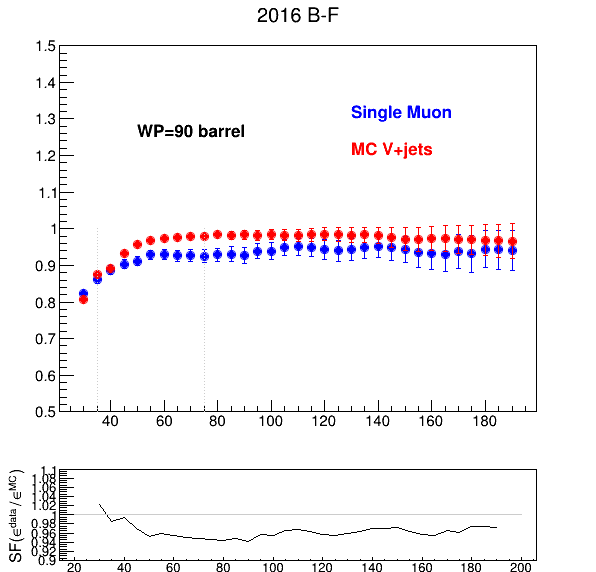
\includegraphics[width=\textwidth]{figures/misc/PhotonFromData_RhoCat12016_WP90_barrel.png}
				\caption{VBF trigger photon-leg efficiencies for MC and data.}
			\end{subfigure}%
			\hfill
			\begin{subfigure}[t]{0.31\linewidth}
				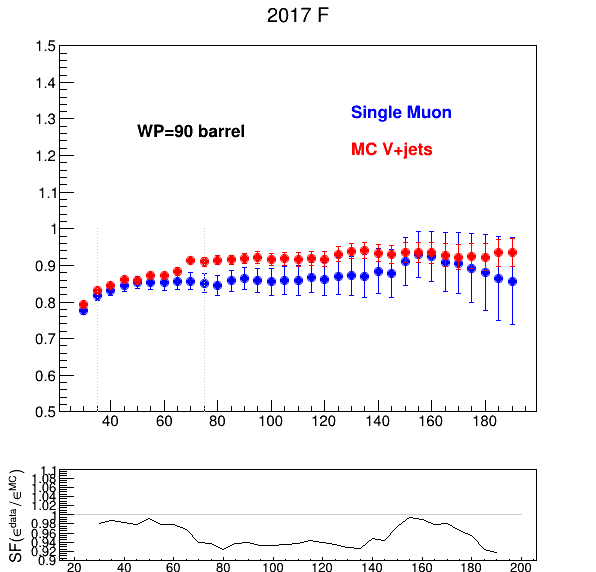
\includegraphics[width=\textwidth]{figures/misc/PhotonFromData_RhoCat2017_WP90_barrel.png}
			\end{subfigure}%
			\hfill
			\begin{subfigure}[t]{0.31\linewidth}
				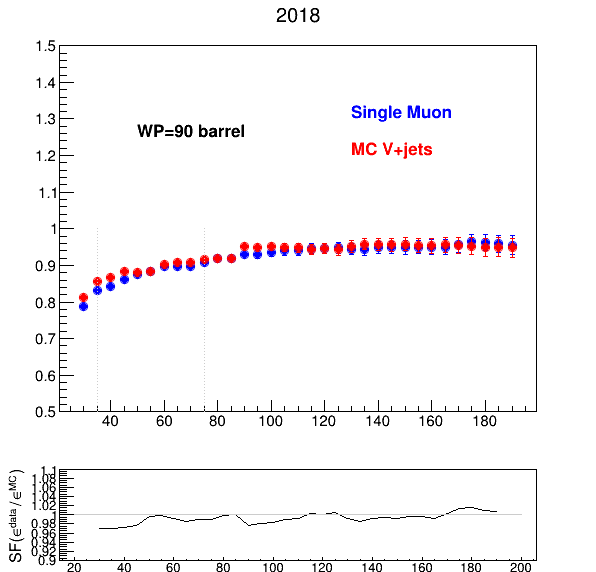
\includegraphics[width=\textwidth]{figures/misc/PhotonFromData_RhoCat2018_WP90_barrel.png}
			\end{subfigure}
			\caption{VBF-dedicated trigger photon-leg efficiencies for MC and data, shown for the \(\Hgrho\) channel in 2016 (top-left), 2017 (top-right), and 2018 (bottom).}
		\end{figure}
	\end{itemize}
\end{frame}

% Isolation scale factors
\begin{frame}{Di-track Isolation Scale Factors}
	
	{\footnotesize This slide was presented during the unblinding talk.}
	\begin{figure}
		\centering
		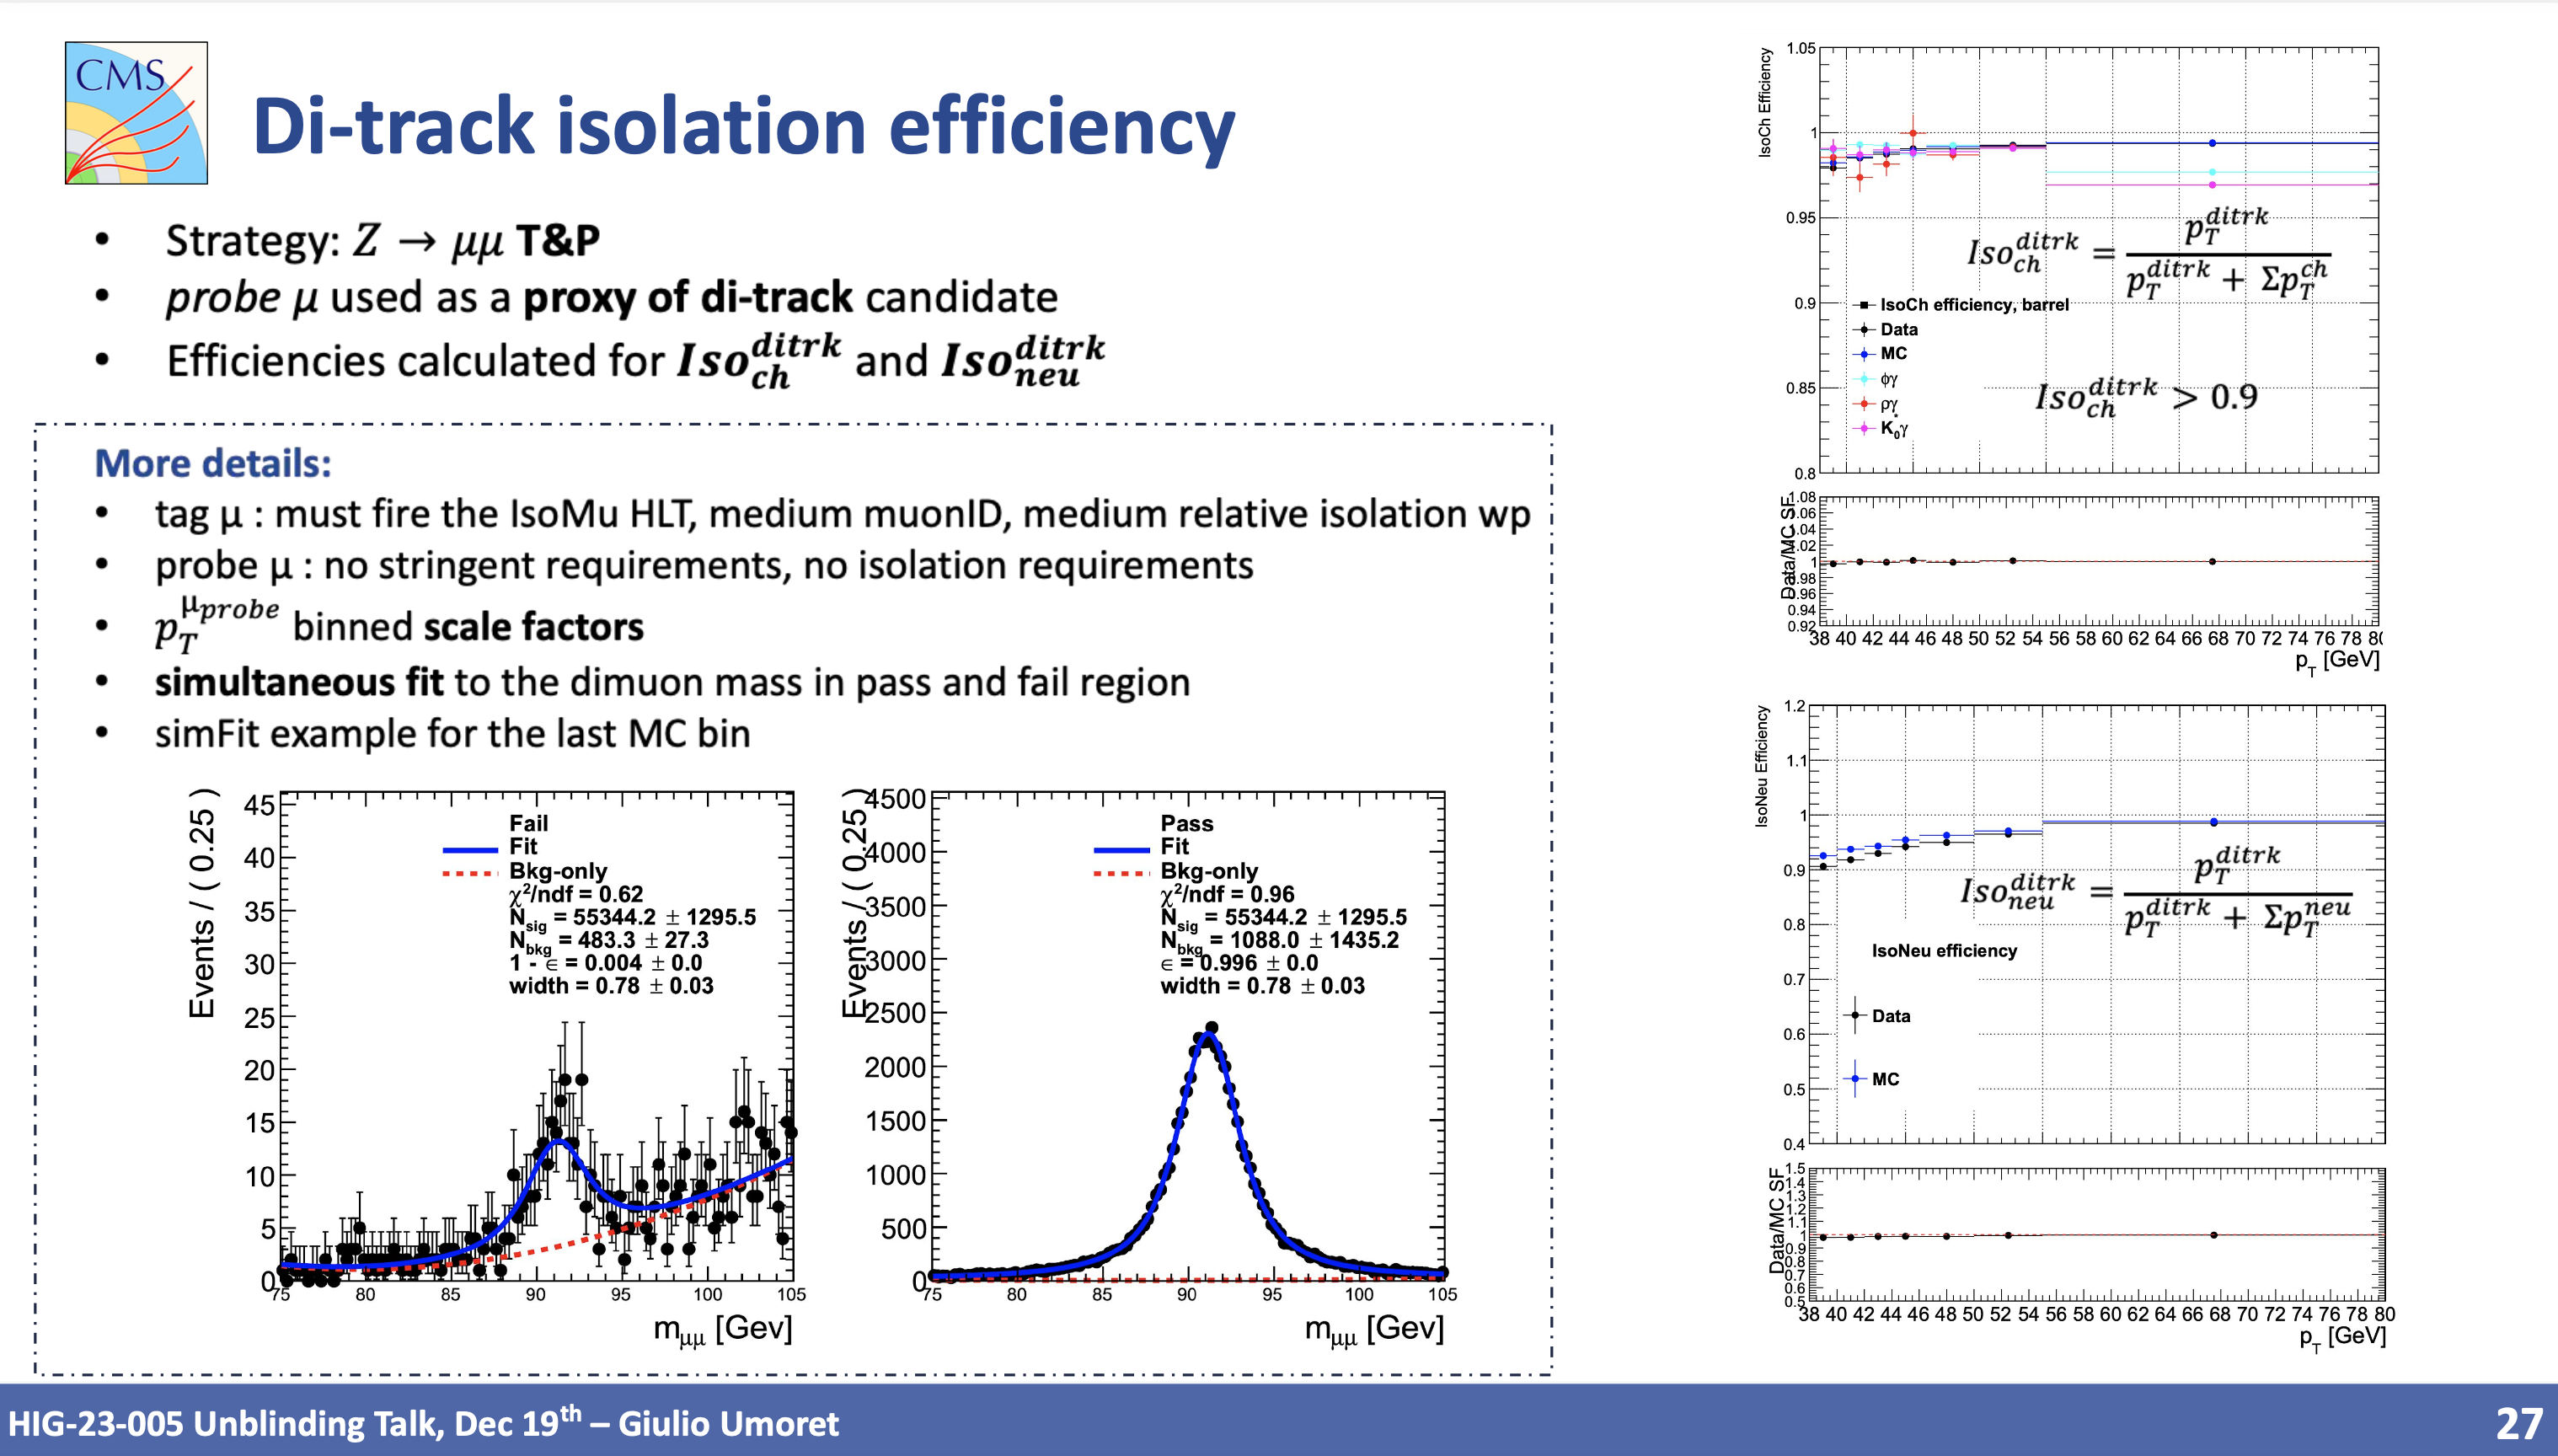
\includegraphics[height=0.8\textheight]{figures/backup/isolation_scale_factors.png}
	\end{figure}
\end{frame}

% Neutral iso
\begin{frame}{Background Estimation ggG}
	
	{\footnotesize This slide was presented during the unblinding talk.}
	\begin{figure}
		\centering
		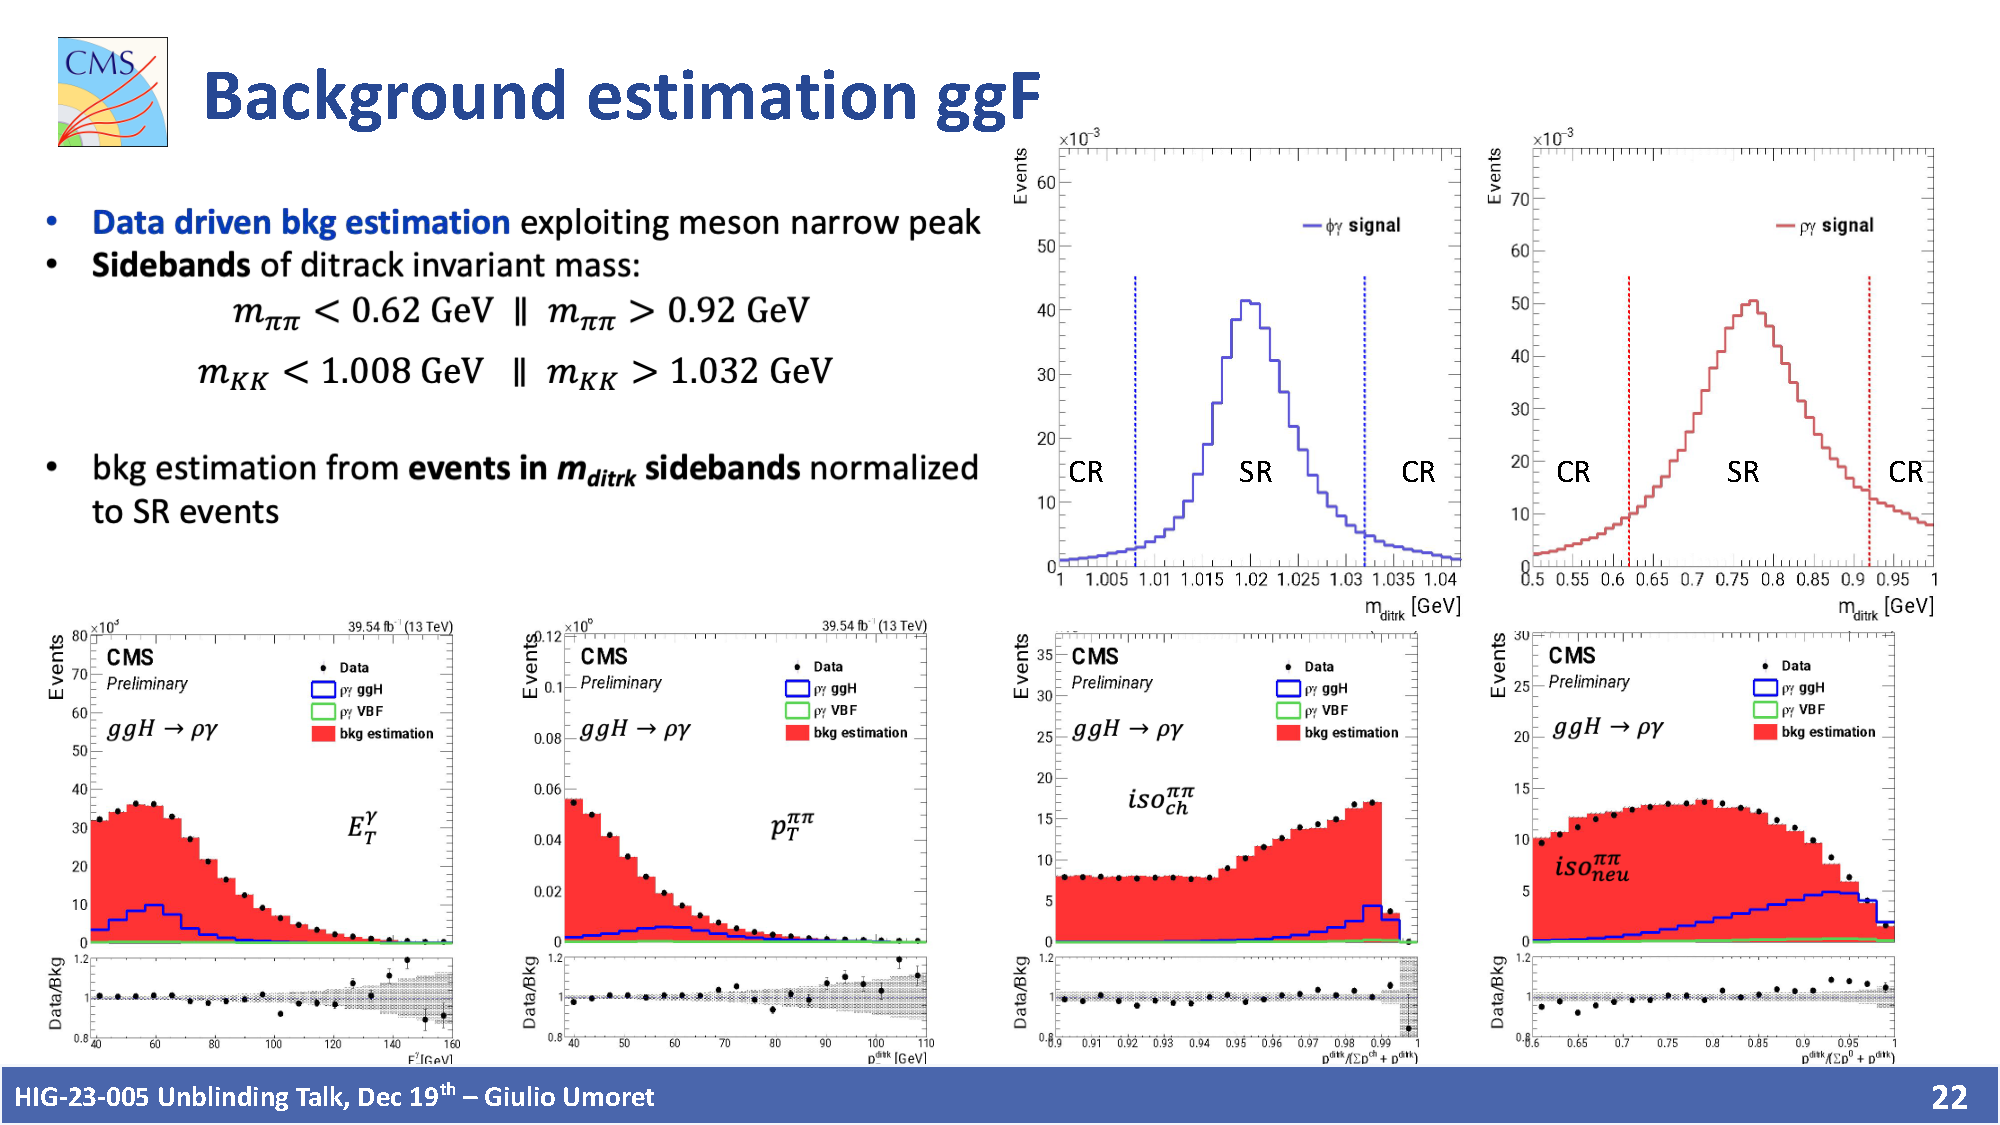
\includegraphics[height=0.8\textheight]{figures/backup/BDT_ggH_bkg_SFs.pdf}
	\end{figure}
\end{frame}

% Meson mass resolution
\begin{frame}{Meson Mass Resolution}
	\label{fr:mesmassres}
	\begin{table}
		\small
		\begin{tabular}{ l | c | c | c }
			Meson & Resolution from \(\mathrm{m^{reco}_{ditrk} - m^{gen}_{ditrk}}\) fit (MeV) & Width from \(\mathrm{m^{reco}_{ditrk}}\) plot (MeV) & Width from PDG (MeV) \\
			\hline
			\(\PGrz\) & 8.89 & 90 & 147\\
			\(\PGf\) & 2.22 & 6.4 & 4.25 \\
			\(\PKstarz\) & 6.08 & 42 & 41 \\
			\hline
		\end{tabular}
	\end{table}
	\begin{figure}
		\begin{subfigure}[t]{0.31\textwidth}
			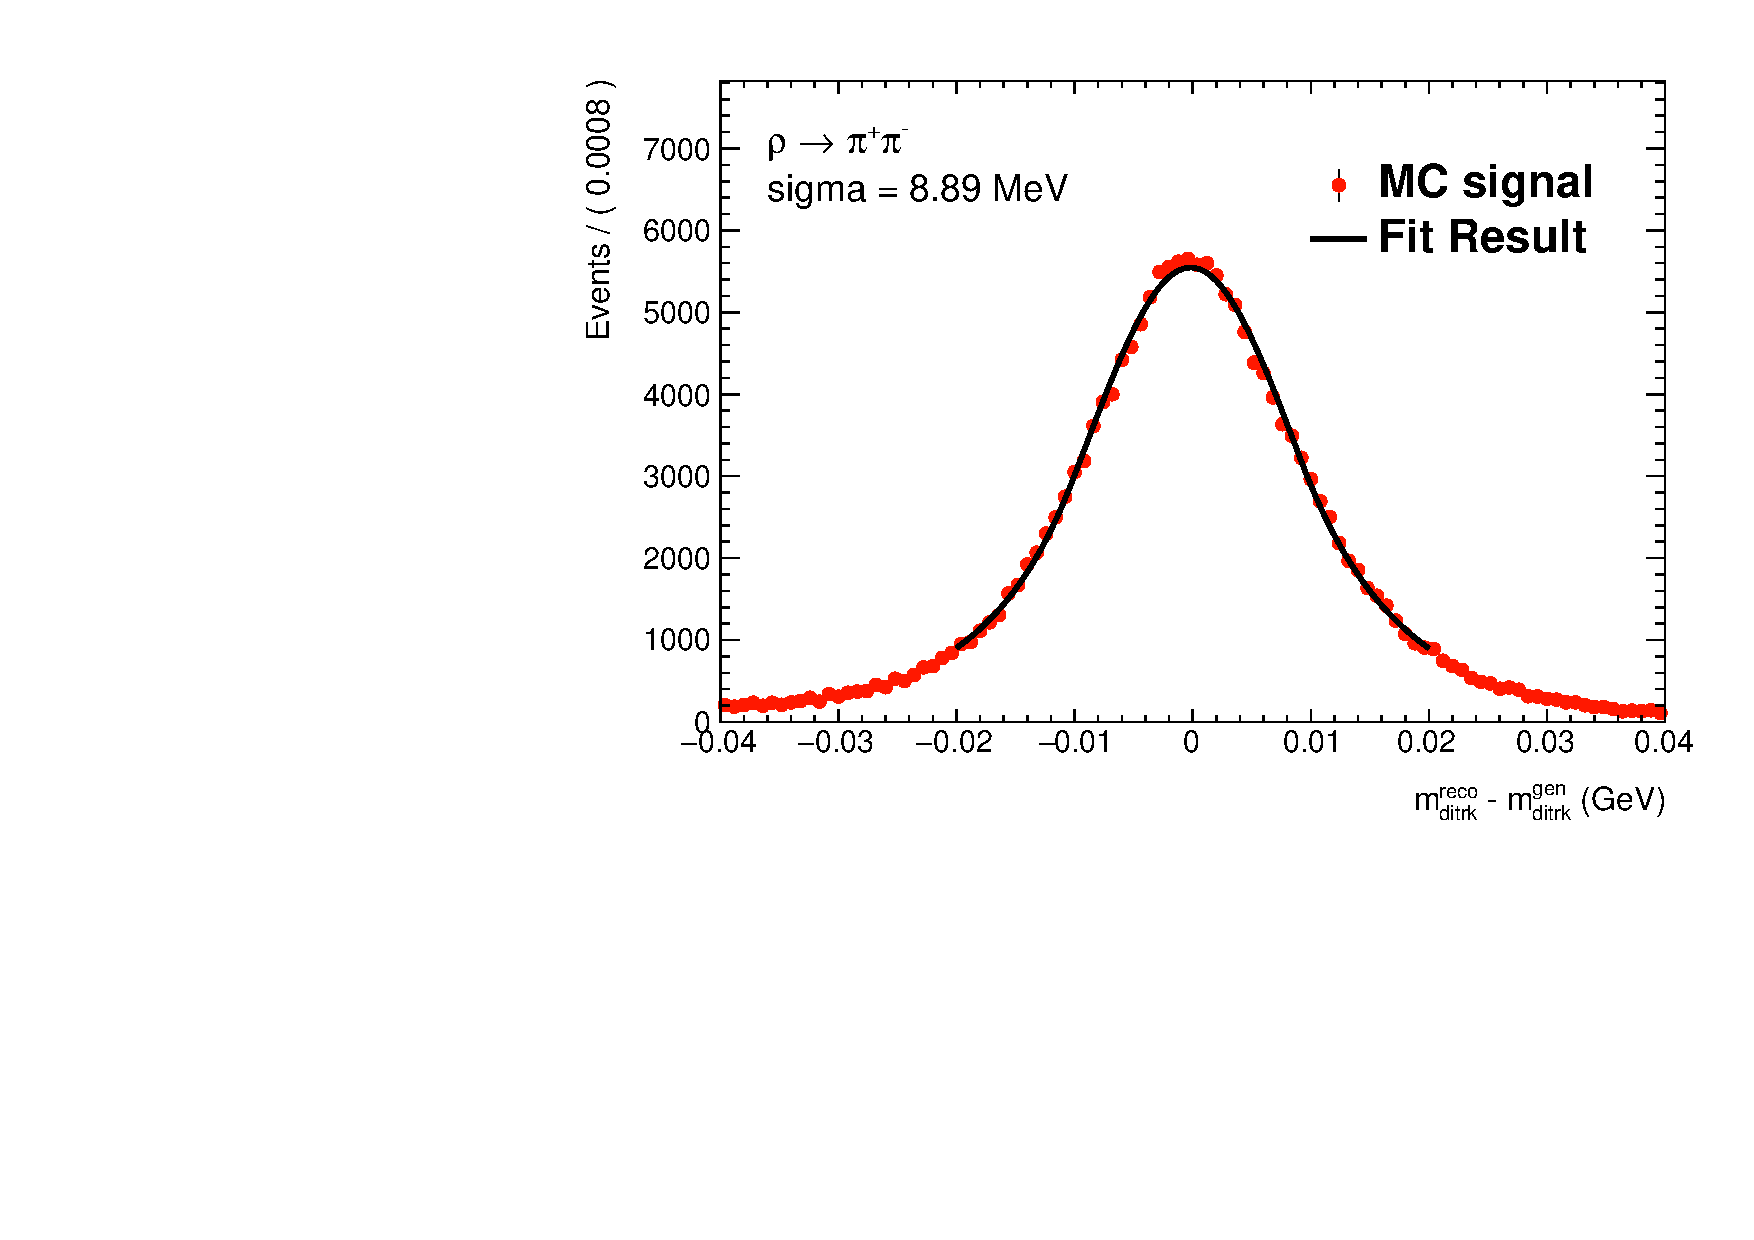
\includegraphics[width=\textwidth]{figures/backup/m_ditrk_Rho_signal.pdf}
			\caption*{\(\Hgrho\)}
		\end{subfigure}%
		\begin{subfigure}[t]{0.31\textwidth}
			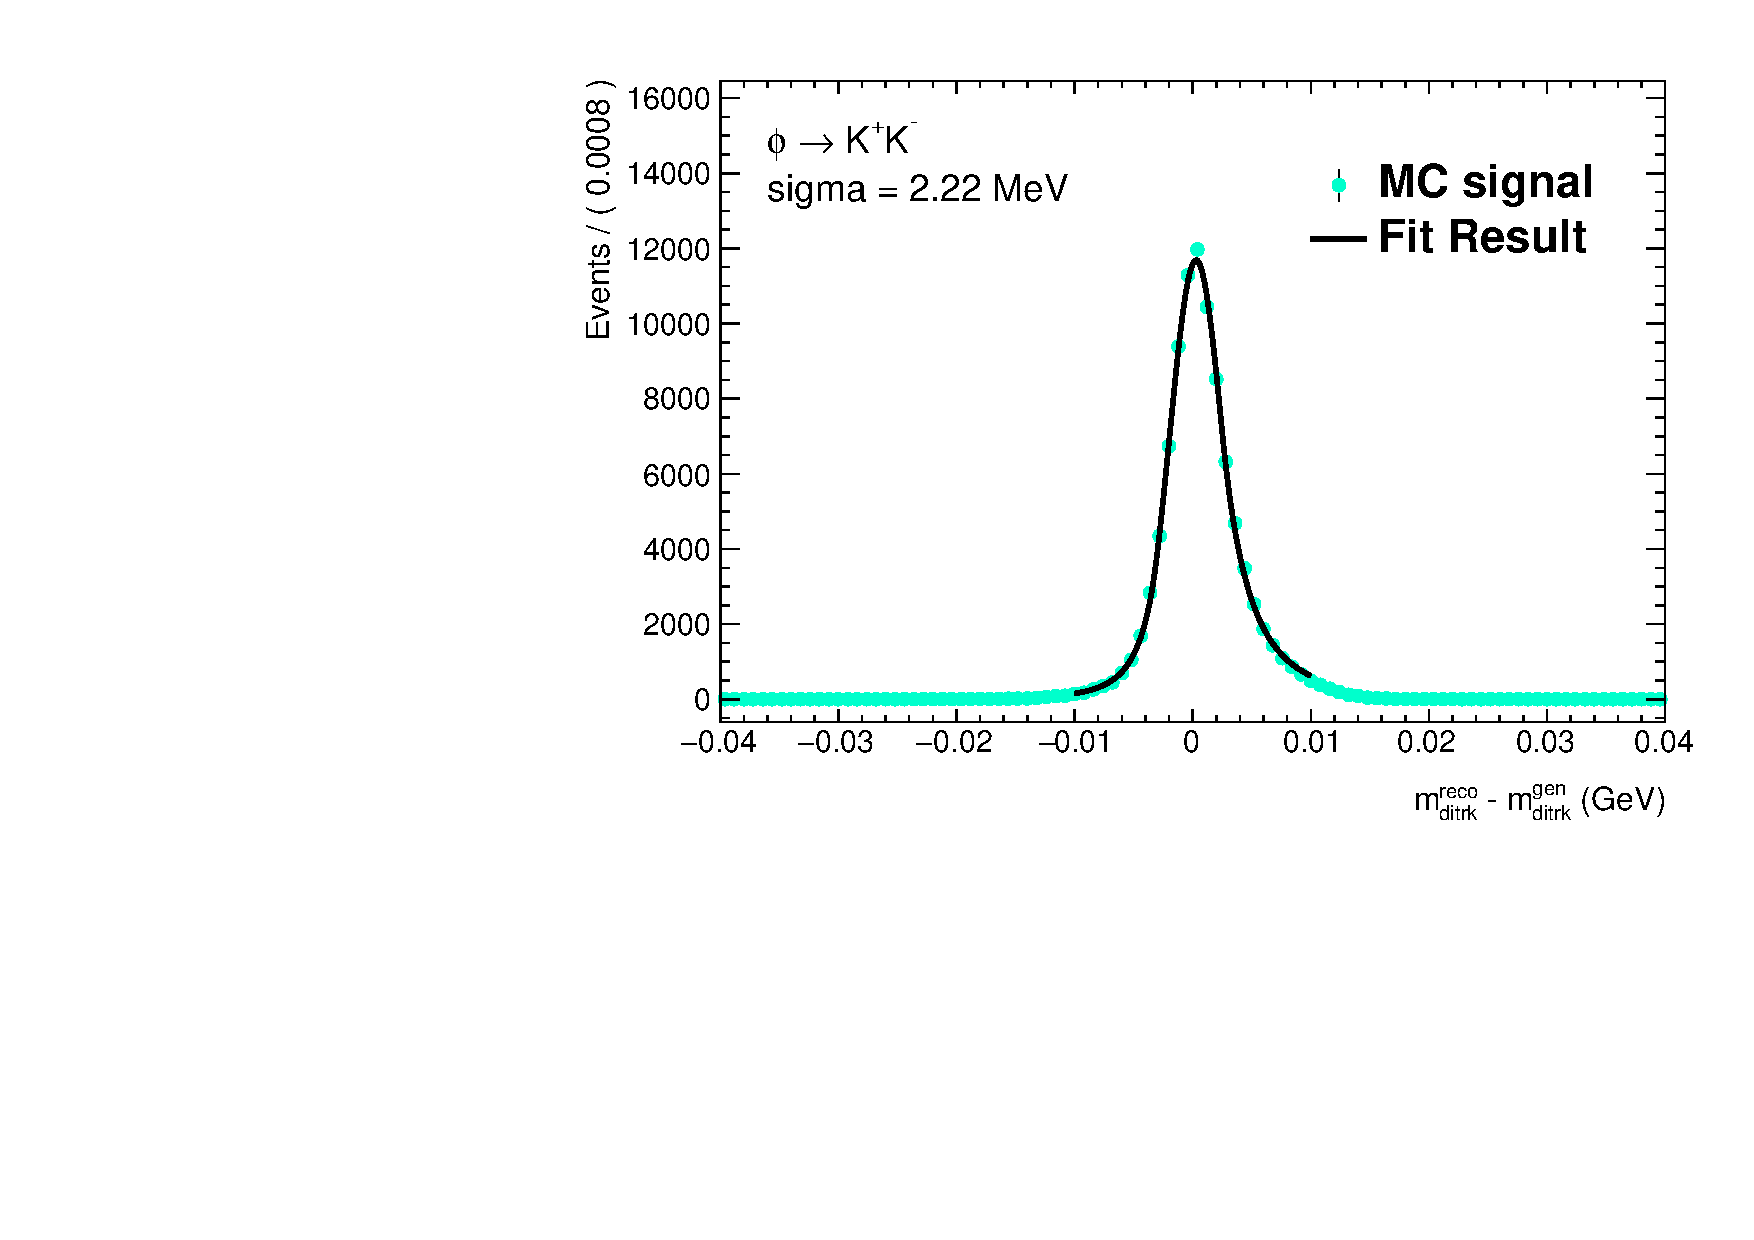
\includegraphics[width=\textwidth]{figures/backup/m_ditrk_Phi_signal.pdf}
			\caption*{\(\Hgphi\)}
		\end{subfigure}%
		\begin{subfigure}[t]{0.31\textwidth}
			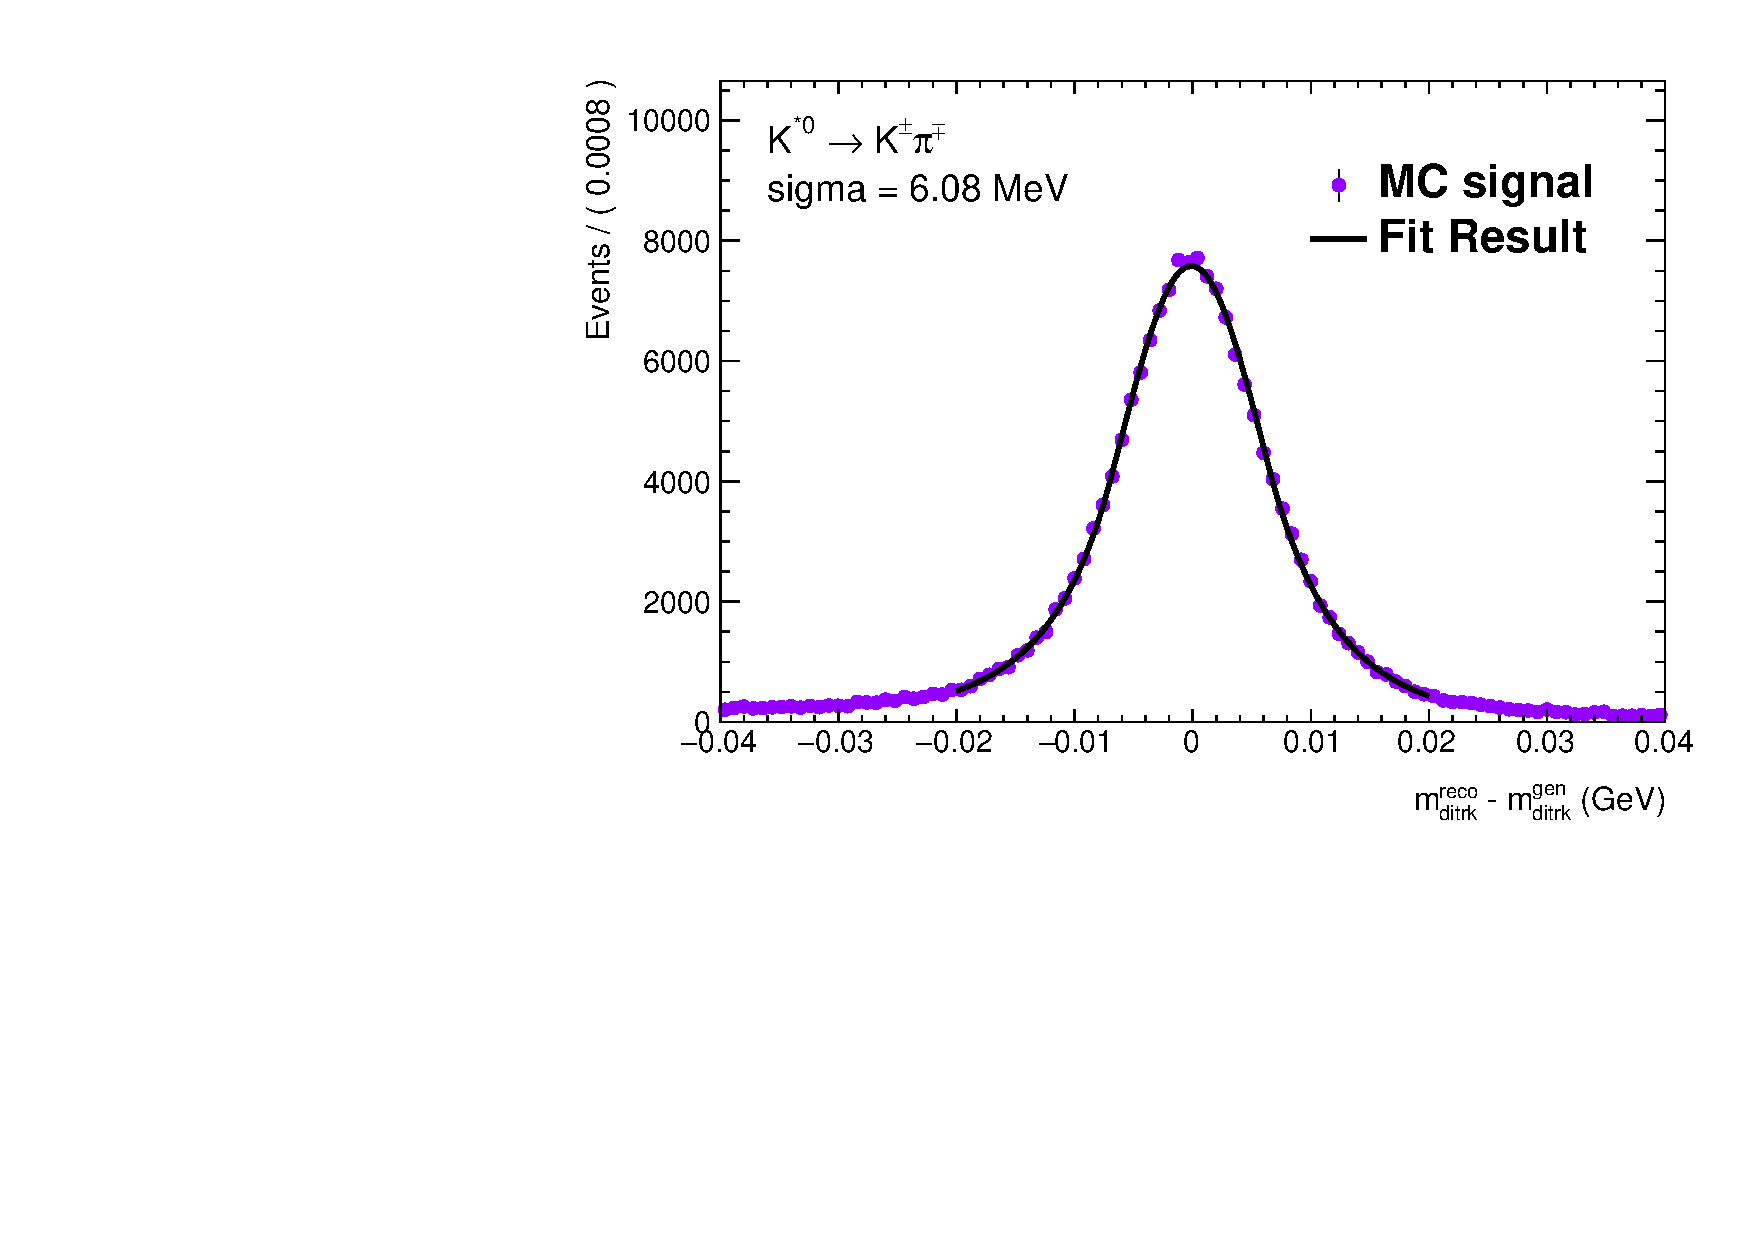
\includegraphics[width=\textwidth]{figures/backup/m_ditrk_K0s_signal.pdf}
			\caption*{\(\Hgkstar\)}
		\end{subfigure}%
		\caption{\(\mathrm{m^{reco}_{ditrk} - m^{gen}_{ditrk}}\)  and Gaussian fit shown for the three decay channels.}
	\end{figure}
\end{frame}

% Systematic impacts (AN-23-004)
%%% Asymmetry problem

\begin{frame}{References}
	\label{fr:refs}
	\scriptsize
	\bibliographystyle{JHEP}
	\bibliography{refs.bib}
\end{frame}
\end{document}
